\documentclass[t]{beamer}
\usetheme{default}
\usepackage{microtype}
\usepackage{tikz}
\usepackage{pgfpages}
\usepackage{listings}
\usepackage{xcolor}
\usepackage{graphicx}
\usepackage{changepage}
%\usepackage{transparent}
\usepackage[normalem]{ulem}
\usepackage{braket}
\usepackage{adjustbox}
\usepackage{appendixnumberbeamer}

\usetikzlibrary{arrows, tikzmark, shadows, calc, matrix, positioning}
% Allows for line numbers in a listing to be referenced in tikz
\usetikzmarklibrary{listings}


\setbeameroption{show notes on second screen=right}
%\setbeameroption{hide notes}
\setbeamertemplate{note page}[plain]
\setbeamerfont{note page}{size=\footnotesize}

% Change itemize graphic from ball to triangle
\setbeamertemplate{itemize items}[triangle]
% Change enumerate graphic to default (colored numbers)
\setbeamertemplate{enumerate items}[default]
% Remove shadows on theroms
\setbeamertemplate{blocks}[rounded][shadow=false]
% Remove shadows on title
\setbeamertemplate{title page}[default][colsep=-4bp,rounded=true]
% Remove shadows on theorems
\setbeamertemplate{blocks}[rounded][shadow=false]
%\setbeamercolor{block title}{fg=structure,bg=white}
\setbeamertemplate{navigation symbols}{} % remove navigation symbols

% Setup beamer colors
\definecolor{mygreen}{rgb}{0,0.6,0}
\definecolor{mygray}{rgb}{0.5,0.5,0.5}
\definecolor{mymauve}{rgb}{0.58,0,0.82}

% Define colors for the theme
%\definecolor{foreground}{RGB}{255,255,255}
%\definecolor{background}{RGB}{24,24,24}
% Lighter colors
\definecolor{background}{RGB}{228,241,254}
\definecolor{title}{RGB}{34,167,240}
\definecolor{foreground}{RGB}{34,49,63}
\definecolor{subtitle}{RGB}{232,126,4}
\definecolor{hilight}{RGB}{31,58,147}
\definecolor{vhilight}{RGB}{255,111,207}
\definecolor{gray}{RGB}{149,165,166}
\definecolor{sandstorm}{RGB}{249, 191, 59}
\definecolor{ggreen}{RGB}{135,211,124}
\definecolor{snuff}{RGB}{220, 198, 224}


% more pastel colors
\definecolor{darkyblue}{HTML}{203F54}
\definecolor{sandy}{HTML}{F7F6F6}
\definecolor{seablue}{HTML}{508EBF}
\definecolor{skyblue}{HTML}{CCDBEA}
\definecolor{cherrypink}{HTML}{DC97A5}


% Material Colors 200
%http://materialuicolors.co/
\definecolor{matred}{HTML}{EF9A9A}
\definecolor{matred400}{HTML}{EF5350}
\definecolor{matblue400}{HTML}{42A5F5}
\definecolor{matpink}{HTML}{F48FB1}
\definecolor{matpink400}{HTML}{EC407A}
\definecolor{matpurp}{HTML}{CE93D8}
\definecolor{matdeeppurp}{HTML}{B39DDB}
\definecolor{matlb100}{HTML}{B3E5FC}
\definecolor{matlb}{HTML}{81D4FA}
\definecolor{matorange}{HTML}{FFCC80}
\definecolor{matorange400}{HTML}{FFA726}
\definecolor{matorange600}{HTML}{FB8C00}
\definecolor{matorange700}{HTML}{F57C00}
\definecolor{matdeeporange}{HTML}{FFAB91}
\definecolor{matdeeporange400}{HTML}{FF7043}
\definecolor{matbluegray}{HTML}{B0BEC5}
\definecolor{matbluegray400}{HTML}{78909C}
\definecolor{matbluegray900}{HTML}{263238}
\definecolor{matindigo}{HTML}{9FA8DA}
\definecolor{matamber400}{HTML}{FFCA28}
\definecolor{matyellow400}{HTML}{FFEE58}
\definecolor{matgray900}{HTML}{212121}

\definecolor{matindigo500}{HTML}{3F51B5}
\definecolor{matindigo400}{HTML}{5C6BC0}


% Material colors
\setbeamercolor{titlelike}{fg=matorange400}
\setbeamercolor{subtitle}{fg=matpink400}
\setbeamercolor{institute}{fg=matbluegray400}
%\setbeamercolor{normal text}{fg=matindigo500,bg=matlb100}
\setbeamercolor{normal text}{fg=matbluegray900,bg=matlb100}
\setbeamercolor{alerted text}{fg=matpink400}
%
\setbeamercolor{item}{fg=matred400} % color of bullets
\setbeamercolor{subitem}{fg=matbluegray900}
\setbeamercolor{itemize/enumerate subbody}{fg=matbluegray900}

\setbeamercolor{section in toc}{fg=matbluegray900}
\setbeamercolor{subsection in toc}{fg=matbluegray900}

% Dark colors
%\definecolor{foreground}{RGB}{255,255,255}
%\definecolor{background}{RGB}{24,24,24}
%\definecolor{title}{RGB}{107,174,214}
%\definecolor{gray}{RGB}{155,155,155}
%\definecolor{subtitle}{RGB}{102,255,204}
%\definecolor{hilight}{RGB}{102,255,204}
%\definecolor{vhilight}{RGB}{255,111,207}

% Setup beamer colors
%\setbeamercolor{titlelike}{fg=title}
%\setbeamercolor{subtitle}{fg=subtitle}
%\setbeamercolor{institute}{fg=gray}
%\setbeamercolor{normal text}{fg=foreground,bg=background}
%\setbeamercolor{alerted text}{fg=subtitle}
%
%\setbeamercolor{item}{fg=title} % color of bullets
%\setbeamercolor{subitem}{fg=gray}
%\setbeamercolor{itemize/enumerate subbody}{fg=foreground}
%
%\setbeamercolor{item}{fg=title} % color of bullets
%\setbeamercolor{subitem}{fg=gray}
%\setbeamercolor{itemize/enumerate subbody}{fg=foreground}
%%%%
%\setbeamertemplate{itemize subitem}{{\textendash}}
%\setbeamerfont{itemize/enumerate subbody}{size=\footnotesize}
%\setbeamerfont{itemize/enumerate subitem}{size=\footnotesize}
% End beamer colors

% Slide number  in lower right in gray
\setbeamertemplate{footline}{%
      \raisebox{5pt}{\makebox[\paperwidth]{\hfill\makebox[20pt]{\color{gray}
                      \scriptsize\insertframenumber/\inserttotalframenumber}}}\hspace*{5pt}}


% Increase the width of slide material used within
% \Wider{...}
\newcommand\Wider[2][3em]{%
\makebox[\linewidth][c]{%
  \begin{minipage}{\dimexpr\textwidth+#1\relax}
  \raggedright#2
  \end{minipage}%
  }%
}


% Listings options
\lstset{ %
	backgroundcolor=\color{background},   % choose the background color; you must add \usepackage{color} or \usepackage{xcolor}
  basicstyle=\small\ttfamily\color{foreground},  % the size of the fonts that are used for the code
	breakatwhitespace=false,         % sets if automatic breaks should only happen at whitespace
	breaklines=true,                 % sets automatic line breaking
	captionpos=b,                    % sets the caption-position to bottom
	commentstyle=\color{gray},    % comment style
	deletekeywords={...},            % if you want to delete keywords from the given language
  escapeinside={(*}{*)},          % if you want to add LaTeX within your code
	extendedchars=true,              % lets you use non-ASCII characters; for 8-bits encodings only, does not work with UTF-8
	frame=none,                    % adds a frame around the code
	keepspaces=true,                 % keeps spaces in text, useful for keeping indentation of code (possibly needs columns=flexible)
	keywordstyle=\color{hilight},    % keyword style
	morekeywords={*,...},            % if you want to add more keywords to the set
	numbers=none,                    % where to put the line-numbers; possible values are (none, left, right)
	numbersep=9pt,                   % how far the line-numbers are from the code
	numberstyle=\color{foreground},       % the style that is used for the line-numbers
	rulecolor=\color{foreground},         % if not set, the frame-color may be changed on line-breaks within not-black text (e.g. comments (green here))
	showspaces=false,                % show spaces everywhere adding particular underscores; it overrides 'showstringspaces'
	showstringspaces=false,          % underline spaces within strings only
	showtabs=false,                  % show tabs within strings adding particular underscores
	stepnumber=1,                    % the step between two line-numbers. If it's 1, each line will be numbered
	stringstyle=\color{vhilight},     % string literal style
	tabsize=3,                       % sets default tabsize to 2 spaces
	%title=\lstname,                   % show the filename of files included with \lstinputlisting; also try caption instead of title
	linewidth=\linewidth,
  % Style of line numbers
  numberstyle=\small\color{gray},
  % Color text red surrounded by @
  %moredelim=**[is][\color{red}]{@}{@},
  language=C
}



% https://tex.stackexchange.com/a/119355
% #1 is the diameter of the circle
% #2--#5 are the colors of each region
\newcommand\DrawCirc[5]{%
\fill[#2] (0,0) arc[radius=0.5*#1,start angle=180,end angle=90] -- +(0,-0.5*#1) --cycle;
\fill[#3] (#1,0) arc[radius=0.5*#1,start angle=0,end angle=90] -- +(0,-0.5*#1) --cycle;
\fill[#4] (#1,0) arc[radius=0.5*#1,start angle=0,end angle=-90] -- +(0,0.5*#1) -- cycle;
\fill[#5] (0.5*#1,-0.5*#1) arc[radius=0.5*#1,start angle=-90,end angle=-180] -- +(0.5*#1,0) -- cycle;
\draw (0.5*#1,0) circle [radius=0.5*#1];

\draw (0,0) -- +(#1,0);
\draw (0.5*#1,-0.5*#1) -- +(0,#1);
}

\newcommand\DrawSquare[3][]{%
\node[inner sep=0pt,outer sep=0pt,draw,rectangle,minimum size=#2,#1] (#3) {}; 
}

\newcommand\DrawSquareOpac[3][]{%
\node[inner sep=0pt,outer sep=0pt,draw,rectangle,minimum size=#2,#1,opacity=0.2] (#3) {}; 
}

\newcommand\FillSquare[3]{%
\ifnum#2=1\relax
  \fill[#3] ( $ (#1.north west) + (0.5\pgflinewidth,-0.5\pgflinewidth) $ ) rectangle (#1.center);
\else
\ifnum#2=2\relax
  \fill[#3] (#1.center) rectangle ( $ (#1.north east) + (-0.5\pgflinewidth,-0.5\pgflinewidth) $ );
\else
\ifnum#2=3\relax
  \fill[#3] ( $ (#1.south west) + (0.5\pgflinewidth,0.5\pgflinewidth) $ ) rectangle (#1.center);
\else
\ifnum#2=4\relax
  \fill[#3] (#1.center) rectangle ( $ (#1.south east) + (-0.5\pgflinewidth,0.5\pgflinewidth) $ );
\fi\fi\fi\fi%
}

\newcommand\FillSquareOpac[3]{%
\ifnum#2=1\relax
  \fill[#3,opacity=0.2] ( $ (#1.north west) + (0.5\pgflinewidth,-0.5\pgflinewidth) $ ) rectangle (#1.center);
\else
\ifnum#2=2\relax
  \fill[#3,opacity=0.2] (#1.center) rectangle ( $ (#1.north east) + (-0.5\pgflinewidth,-0.5\pgflinewidth) $ );
\else
\ifnum#2=3\relax
  \fill[#3,opacity=0.2] ( $ (#1.south west) + (0.5\pgflinewidth,0.5\pgflinewidth) $ ) rectangle (#1.center);
\else
\ifnum#2=4\relax
  \fill[#3,opacity=0.2] (#1.center) rectangle ( $ (#1.south east) + (-0.5\pgflinewidth,0.5\pgflinewidth) $ );
\fi\fi\fi\fi%
}

\newcommand\LabelRegion[3]{%
\ifnum#2=1\relax
\node at ( $ (#1.north west)!0.5!(#1.center) $ ) {#3};
\else
\ifnum#2=2\relax
\node at ( $ (#1.north east)!0.5!(#1.center) $ ) {#3};
\else
\ifnum#2=3\relax
\node at ( $ (#1.south west)!0.5!(#1.center) $ ) {#3};
\else
\ifnum#2=4\relax
\node at ( $ (#1.south east)!0.5!(#1.center) $ ) {#3};
\fi\fi\fi\fi%
}

\newcommand\LabelRegionOpac[3]{%
\ifnum#2=1\relax
\node[opacity=0.2] at ( $ (#1.north west)!0.5!(#1.center) $ ) {#3};
\else
\ifnum#2=2\relax
\node[opacity=0.2] at ( $ (#1.north east)!0.5!(#1.center) $ ) {#3};
\else
\ifnum#2=3\relax
\node[opacity=0.2] at ( $ (#1.south west)!0.5!(#1.center) $ ) {#3};
\else
\ifnum#2=4\relax
\node[opacity=0.2] at ( $ (#1.south east)!0.5!(#1.center) $ ) {#3};
\fi\fi\fi\fi%
}

% #4 is the frame on which the label is visible
\newcommand\LabelRegionVis[4]{%
\ifnum#2=1\relax
\node[visible on=#4] at ( $ (#1.north west)!0.5!(#1.center) $ ) {#3};
\else
\ifnum#2=2\relax
\node[visible on=#4] at ( $ (#1.north east)!0.5!(#1.center) $ ) {#3};
\else
\ifnum#2=3\relax
\node[visible on=#4] at ( $ (#1.south west)!0.5!(#1.center) $ ) {#3};
\else
\ifnum#2=4\relax
\node[visible on=#4] at ( $ (#1.south east)!0.5!(#1.center) $ ) {#3};
\fi\fi\fi\fi%
}

\newcommand\LabelRegionSmall[3]{%
\ifnum#2=1\relax
\node[yshift=-0.5cm] at ( $ (#1.north west)!0.5!(#1.center) $ ) {\tiny#3};
\else
\ifnum#2=2\relax
\node[yshift=-0.5cm] at ( $ (#1.north east)!0.5!(#1.center) $ ) {\tiny#3};
\else
\ifnum#2=3\relax
\node[yshift=-0.5cm] at ( $ (#1.south west)!0.5!(#1.center) $ ) {\tiny#3};
\else
\ifnum#2=4\relax
\node[yshift=-0.5cm] at ( $ (#1.south east)!0.5!(#1.center) $ ) {\tiny#3};
\fi\fi\fi\fi%
}

\newcommand\LabelRegionSmallOpac[3]{%
\ifnum#2=1\relax
\node[opacity=0.2,yshift=-0.5cm] at ( $ (#1.north west)!0.5!(#1.center) $ ) {\tiny#3};
\else
\ifnum#2=2\relax
\node[opacity=0.2,yshift=-0.5cm] at ( $ (#1.north east)!0.5!(#1.center) $ ) {\tiny#3};
\else
\ifnum#2=3\relax
\node[opacity=0.2,yshift=-0.5cm] at ( $ (#1.south west)!0.5!(#1.center) $ ) {\tiny#3};
\else
\ifnum#2=4\relax
\node[opacity=0.2,yshift=-0.5cm] at ( $ (#1.south east)!0.5!(#1.center) $ ) {\tiny#3};
\fi\fi\fi\fi%
}

\newcommand\LabelRegionSmallVis[4]{%
\ifnum#2=1\relax
\node[visible on=#4, yshift=-0.5cm] at ( $ (#1.north west)!0.5!(#1.center) $ ) {\tiny#3};
\else
\ifnum#2=2\relax
\node[visible on=#4, yshift=-0.5cm] at ( $ (#1.north east)!0.5!(#1.center) $ ) {\tiny#3};
\else
\ifnum#2=3\relax
\node[visible on=#4, yshift=-0.5cm] at ( $ (#1.south west)!0.5!(#1.center) $ ) {\tiny#3};
\else
\ifnum#2=4\relax
\node[visible on=#4, yshift=-0.5cm] at ( $ (#1.south east)!0.5!(#1.center) $ ) {\tiny#3};
\fi\fi\fi\fi%
}

\newcommand\DrawLines[1]{%
\draw (#1.north) -- (#1.south);
\draw (#1.west) -- (#1.east);
}

% Keys to support piece-wise uncovering of elements in TikZ pictures:
% \node[visible on=<2->](foo){Foo}
% \node[visible on=<{2,4}>](bar){Bar}   % put braces around comma expressions
%
% Internally works by setting opacity=0 when invisible, which has the 
% adavantage (compared to \node<2->(foo){Foo} that the node is always there, hence
% always consumes space that (foo) is always available.
%
% The actual command that implements the invisibility can be overriden
% by altering the style invisible. For instance \tikzsset{invisible/.style={opacity=0.2}}
% would dim the "invisible" parts. Alternatively, the color might be set to white, if the
% output driver does not support transparencies (e.g., PS) 
%
\tikzset{
  invisible/.style={opacity=0},
  visible on/.style={alt={#1{}{invisible}}},
  alt/.code args={<#1>#2#3}{%
    \alt<#1>{\pgfkeysalso{#2}}{\pgfkeysalso{#3}} % \pgfkeysalso doesn't change the path
  },
}

\tikzset{
    % Baloooooon
    incorrect/.style={
    draw,
    fill=red!70,
    text=white,
    rounded corners,
    drop shadow,
    align=left,
  },
}

\tikzstyle{every picture}+=[remember picture]
\tikzset{
    % Baloooooon
    comment/.style={
    draw,
    fill=blue!70,
    text=white,
    rounded corners,
    drop shadow,
    align=left,
  },
}
\tikzset{
  % Graph arrow style (dashed)
  darr/.style={
    line width = 0.4mm
    , dashed
  },
}

\tikzset{
  % Graph arrow style
  garr/.style={
    line width = 0.4mm
  },
}

\tikzset{
  %unreachable statement
  unreach/.style={
    draw
    %, fill=sorange
    %, fill=wax
    , fill=matbluegray400
    %, opacity=0.2
    %, text=white
    , line width=1pt
    , anchor=center
    , text centered
    , rounded corners
    %, minimum width={10em},
    %, minimum height={2em},
    %, rounded corners
  },
}
\tikzset{
  %process node style
  thread/.style={
    draw
    %, fill=sorange
    %, fill=wax
    , fill=matorange400
    %, text=white
    , line width=1pt
    , anchor=center
    , text centered
    , rounded corners
    %, minimum width={10em},
    %, minimum height={2em},
    %, rounded corners
  },
}

\tikzset{
  % Graph arrow style (dashed, red)
  darrc/.style={
    line width = 0.4mm
    , matorange400
    %, dashed
  },
}

\tikzset{
  % generic graph node
  gnode/.style={
    draw
    , line width=1pt
    , fill=ggreen
    %, fill=stree
    , anchor=center
    , text centered
    , rounded corners
  },
}

\tikzset{
  % generic graph node
  gnode2/.style={
    draw
    , line width=1pt
    , fill=snuff
    %, fill=stree
    , anchor=center
    , text centered
    , rounded corners
  },
}

\begin{document}
\title[Constraint AI]{Constraint-Based Thread-Modular Abstract Interpretation}
\author[Kusano]{Markus Kusano}
\institute{Virginia Tech, ECE Department}
\date{XXX DATE XXX}

\begin{frame}
  \maketitle
\end{frame}

\section{Introduction}

\begin{frame}[c]{Intel Speed Racer Bug}

\begin{adjustwidth}{-10.5em}{-10.5em}
\begin{center}
\begin{tikzpicture}
  \node (intel) {
\includegraphics[width=0.4\textwidth]{intel.png}};
  \node [right of=intel, node distance=8cm] (user) {
\includegraphics[width=0.4\textwidth]{maliscious-user.png}};
  %\draw[red, line width=0.25cm, arrows={->[scale=4,blue]}] (intel.east) -- (user.west);
  \draw[visible on=<2->, matred400, line width=0.25cm, arrows={->[scale=4,matblue400]}] (user.west) -- (intel.east);
  %\draw[red, line width=0.25cm, preaction={-triangle 90,thin,draw}] (intel.east) -- (user.west);
\end{tikzpicture}
\end{center}
\end{adjustwidth}

  \note{
    \begin{itemize}
      \item In 2015 a race condition in Intel processors allowed for an
        attacker to perform arbitrary writes to the processors flash memory
      \item This enabled the attackers code to be written directly onto the
        processor, meaning that the maleware would be persistent even across OS
        installations, making this particularly nasty
      \item (Source: https://bromiumlabs.files.wordpress.com/2015/01/speed\_racer\_whitepaper.pdf)
      \item Malicious user source: http://substack.net/
    \end{itemize}
  }
\end{frame}

\begin{frame}{Intel Speed Racer Bug}
  \begin{center}
    \only<1>{
      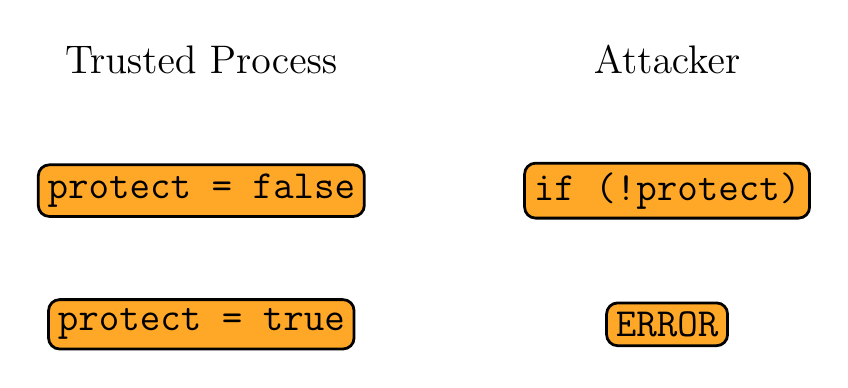
\begin{tikzpicture}
        \matrix (bd) [matrix of nodes
                      , column sep=20mm
                      , row sep=10mm
                      % Beamer messes with everything
                      , ampersand replacement=\&
                     ]
          {
            {\Large Trusted Process}
            \& {\Large Attacker}
            \\
            |[thread]| {\Large \texttt{protect = false}} 
            \& |[thread]| {\Large \texttt{if (!protect)}}
            \\
            |[thread]| {\Large \texttt{protect = true}} 
            \& |[thread]| {\Large \texttt{ERROR}} 
            \\
          }; % matrix
      \end{tikzpicture}
    } %only<1>
    \only<2>{
      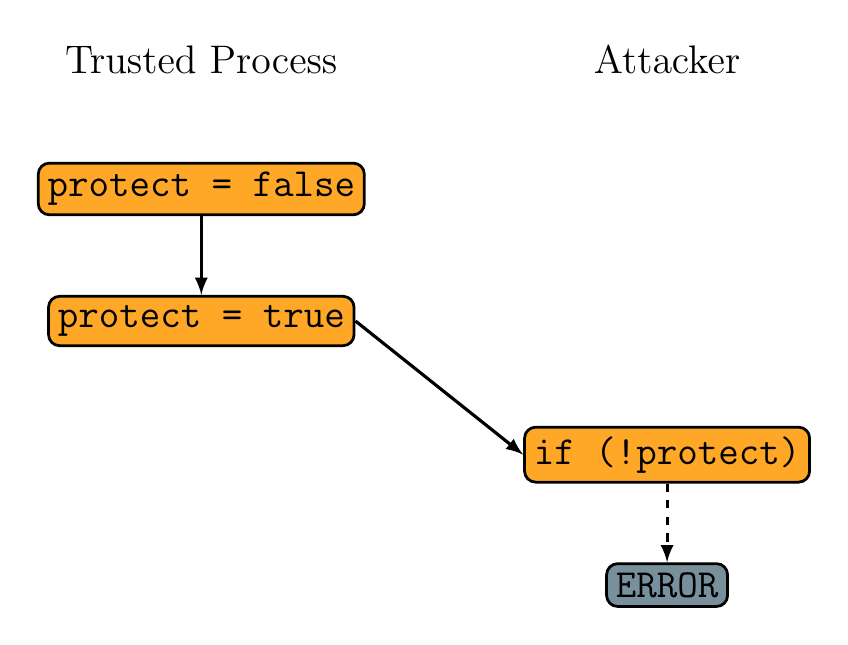
\begin{tikzpicture}
        \matrix (ex1) [matrix of nodes
                      , column sep=20mm
                      , row sep=10mm
                      % Beamer messes with everything
                      , ampersand replacement=\&
                     ]
          {
            {\Large Trusted Process}
            \& {\Large Attacker}
            \\
            |[thread]| {\Large \texttt{protect = false}} %2-1
            \& {}
            \\
            |[thread]| {\Large \texttt{protect = true}} %3-1
            \& {}
            \\
            {}
            \& |[thread]| {\Large \texttt{if (!protect)}} %4-2
            \\
            {}
            \& |[unreach]| {\Large \texttt{ERROR}} %5-2
            \\
          }; % matrix
          \draw[>=latex,->, garr] 
            ($(ex1-2-1.south)$)
            to
            ($(ex1-3-1.north)$);
          \draw[>=latex,->, garr] 
            ($(ex1-3-1.east)$)
            to
            ($(ex1-4-2.west)$);
          \draw[>=latex,->, darr] 
            ($(ex1-4-2.south)$)
            to
            ($(ex1-5-2.north)$);
      \end{tikzpicture}
    } %only<2-9>
    \only<3>{
      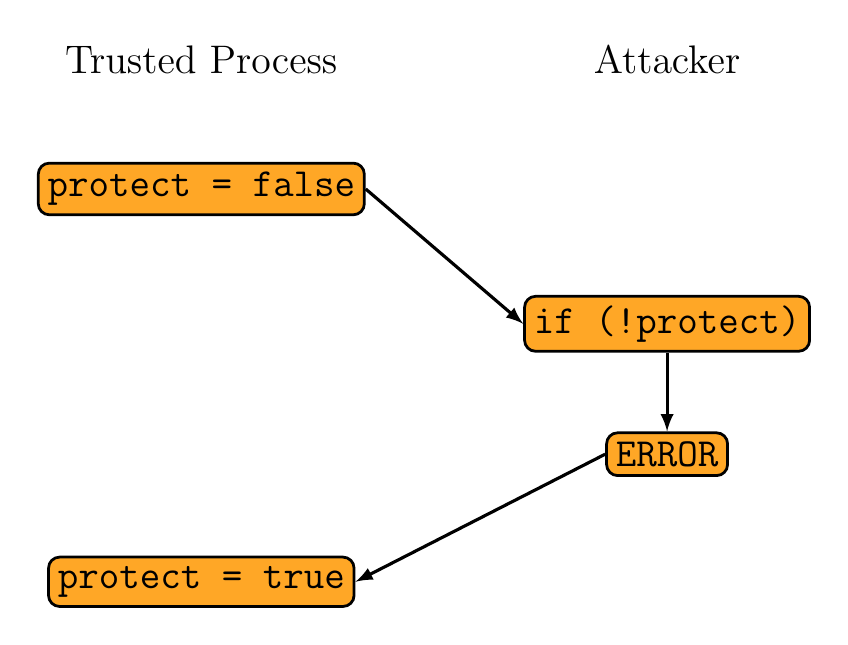
\begin{tikzpicture}
        \matrix (ex1) [matrix of nodes
                      , column sep=20mm
                      , row sep=10mm
                      % Beamer messes with everything
                      , ampersand replacement=\&
                     ]
          {
            {\Large Trusted Process}
            \& {\Large Attacker}
            \\
            |[thread,]| {\Large \texttt{protect = false}} %2-1
            \& {}
            \\
            {}
            \& |[thread,]| {\Large \texttt{if (!protect)}} %4-2
            \\
            {}
            \& |[thread,]| {\Large \texttt{ERROR}} %5-2
            \\
            |[thread,]| {\Large \texttt{protect = true}} %3-1
            \& {}
            \\
          }; % matrix
          \draw[>=latex,->, garr] 
            ($(ex1-2-1.east)$)
            to
            ($(ex1-3-2.west)$);
          \draw[>=latex,->, garr] 
            ($(ex1-3-2.south)$)
            to
            ($(ex1-4-2.north)$);
          \draw[>=latex,->, garr] 
            ($(ex1-4-2.west)$)
            to
            ($(ex1-5-1.east)$);
      \end{tikzpicture}
    } %only<1>
  \end{center}
  \note{
    \begin{itemize}
      \item The Intel bug was caused by a race condition exploited by the
        attacker
      \item At a high-level, the attack involves a trusted process temporarily
        disabling flash write-protection; and an attacker process continuously
        checking if write protection was enabled or not
      \item Typically, the two processes executed where first the trusted
        process running to completion, thereby re-enabling write protection,
        meaning that the attacker process could not do anything malicious
      \item However: there is a small chance that the attacker process
        interleaves with the trusted process
      \item In this case, write-protection is disabled, and the attacker is
        able to execute malicious code and write to the processor's flash
    \end{itemize}
  }
\end{frame}

\begin{frame}[c]{State Explosion}
  %\begin{itemize}[<+->]
  %  \item Lots of thread schedules
  %  \item Hard for a programmer to reason about correctness
  %  \item Hard for a \emph{computer} to reason about correctness
  %  \item Hard to test concurrency bugs traditionally
  %  \item Hard to reproduce concurrency bugs
  %  \item Hard to fix concurrency bugs
  %\end{itemize}

  \begin{center}
    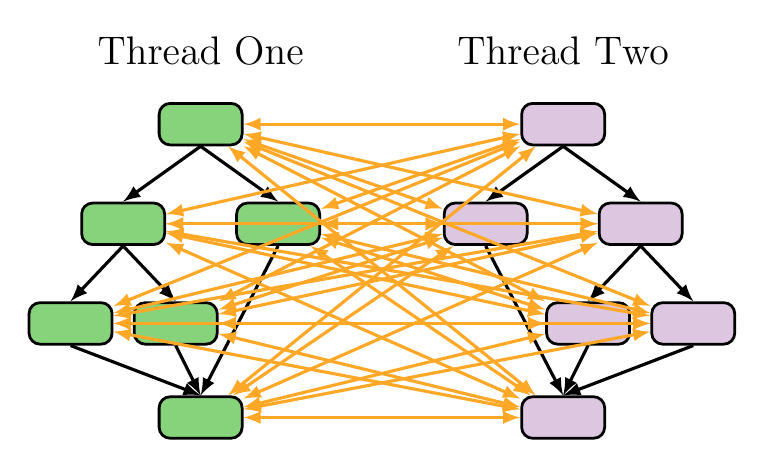
\begin{tikzpicture}
      % Left thread
      \node (ltop) [gnode
                   , minimum width=3em
                   , minimum height=1.5em
                   ] {};
      \node (lml) [gnode
                   , minimum width=3em
                   , minimum height=1.5em
                   , below left=2em and -0.3em of ltop
                   ] {};
      \node (lmlbl) [gnode
                   , minimum width=3em
                   , minimum height=1.5em
                   , below left=2em and -1.2em of lml
                   ] {};
      \node (lmlbr) [gnode
                   , minimum width=3em
                   , minimum height=1.5em
                   , below right=2em and -1.2em of lml
                   ] {};
      \node (lmr) [gnode
                   , minimum width=3em
                   , minimum height=1.5em
                   , below right=2em and -0.3em of ltop
                   ] {};
      \node (lb) [gnode
                   , minimum width=3em
                   , minimum height=1.5em
                   , below=9.0em of ltop
                   ] {};
      \draw[>=latex,->, garr] 
        (ltop.south)
        to
        (lml.north);

      \draw[>=latex,->, garr] 
        (lml.south)
        to
        (lmlbl.north);

      \draw[>=latex,->, garr] 
        (lml.south)
        to
        (lmlbr.north);

      \draw[>=latex,->, garr] 
        (lmlbr.south)
        to
        (lb.north);
      \draw[>=latex,->, garr] 
        (lmlbl.south)
        to
        (lb.north);

      \draw[>=latex,->, garr] 
        (ltop.south)
        to
        (lmr.north);

      \draw[>=latex,->, garr] 
        (lmr.south)
        to
        (lb.north);
  
      % Right thread
      \node (rtop) [gnode2
                   , minimum width=3em
                   , minimum height=1.5em
                   , right =10em of ltop
                   ] {};
      \node (rml) [gnode2
                   , minimum width=3em
                   , minimum height=1.5em
                   , below left=2em and -0.3em of rtop
                   ] {};
      \node (rmr) [gnode2
                   , minimum width=3em
                   , minimum height=1.5em
                   , below right=2em and -0.3em of rtop
                   ] {};
      \node (rmrbl) [gnode2
                   , minimum width=3em
                   , minimum height=1.5em
                   , below left=2em and -1.2em of rmr
                   ] {};
      \node (rmrbr) [gnode2
                   , minimum width=3em
                   , minimum height=1.5em
                   , below right=2em and -1.2em of rmr
                   ] {};
      \node (rb) [gnode2
                   , minimum width=3em
                   , minimum height=1.5em
                   , below=9.0em of rtop
                   ] {};
      \draw[>=latex,->, garr] 
        (rtop.south)
        to
        (rml.north);

      \draw[>=latex,->, garr] 
        (rmr.south)
        to
        (rmrbl.north);

      \draw[>=latex,->, garr] 
        (rmr.south)
        to
        (rmrbr.north);

      \draw[>=latex,->, garr] 
        (rmrbr.south)
        to
        (rb.north);
      \draw[>=latex,->, garr] 
        (rmrbl.south)
        to
        (rb.north);

      \draw[>=latex,->, garr] 
        (rtop.south)
        to
        (rmr.north);

      \draw[>=latex,->, garr] 
        (rml.south)
        to
        %($(rb.north) - (1.0em,0em)$);
        (rb.north);
    % Labels for the two thread
      \node (t1lbl) [above=1em of ltop] {\Large Thread One};
      \node (t2lbl) [above=1em of rtop] {\Large Thread Two};


      %inter-thread edges
      \foreach \NODE in {ltop,lml,lmlbl,lmlbr,lmr,lb}{
        \draw<2->[>=latex,<->, darrc] 
          (\NODE)
          -- 
          %($(rb.north) - (1.0em,0em)$);
          (rtop);
        \draw<2->[>=latex,<->, darrc] 
          (\NODE)
          --
          %($(rb.north) - (1.0em,0em)$);
          (rml);
        \draw<2->[>=latex,<->, darrc] 
          (\NODE)
          --
          %($(rb.north) - (1.0em,0em)$);
          (rmr);
        \draw<2->[>=latex,<->, darrc] 
          (\NODE)
          --
          %($(rb.north) - (1.0em,0em)$);
          (rmrbl);
        \draw<2->[>=latex,<->, darrc] 
          (\NODE)
          --
          %($(rb.north) - (1.0em,0em)$);
          (rmrbr);
        \draw<2->[>=latex,<->, darrc] 
          (\NODE)
          --
          %($(rb.north) - (1.0em,0em)$);
          (rb);
        }%foreach


    \end{tikzpicture}
  \end{center}

  \note{
    \begin{itemize}
      \item The fundamental challenge with concurrent programs are the
        astronomical number of thread schedules: even two simple threads when
        composed concurrently become unwieldy 
      \item There are so many schedulers that a programmer writing a concurrent
        program is unable to reason about them all and notice subtle
        inter-thread interactions
      \item More so, the astronomical number of thread-schedules are even
        difficult for a computer to reason about: the state space grows
        exponentially wrt the number of threads and quickly becomes intractable
      \item Furthermore, traditional testing where you simply run the program
        with user-provided test inputs often fails to find bugs since the
        thread schedule is non-deterministic and typically only explores a
        small fraction of the state space
      \item As a result, even if you know there is a bug lurking in your code
        it can be difficult to reproduce it reliably, and thus makes it hard to
        study and diagnosis the root cause
      \item And, even if you've pinpointed where the bug is, writing a correct
        fix which both completely removes the bug, and does not introduce new
        bugs is very difficult
      \item All of these problems hinder the development of reliable concurrent
        software
    \end{itemize}
  }
\end{frame}


\begin{frame}[fragile,t]

\begin{center}
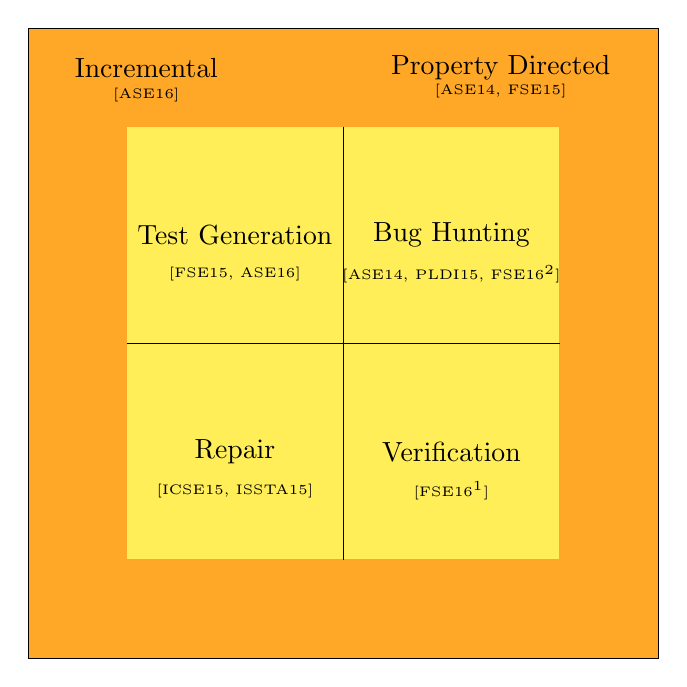
\begin{tikzpicture}
  %  \node [fill=matorange400, draw, thick, shape=rectangle, minimum width=9cm, minimum height=8cm, anchor=center] at (3cm,0) {};
  %\DrawCirc{6cm}{matyellow400}{matyellow400}{matyellow400}{matyellow400}

  \DrawSquare{5.5cm}{in}
  \DrawSquare{8cm}{out}
  \FillSquare{out}{1}{matorange400}
  \FillSquare{out}{2}{matorange400}
  \FillSquare{out}{3}{matorange400}
  \FillSquare{out}{4}{matorange400}

  \FillSquare{in}{1}{matyellow400}
  \FillSquare{in}{2}{matyellow400}
  \FillSquare{in}{3}{matyellow400}
  \FillSquare{in}{4}{matyellow400}

  \DrawLines{in}


  \LabelRegionVis{in}{1}{Test Generation}{<2->}
  \LabelRegionSmallVis{in}{1}{[FSE15, ASE16]}{<2->}

  \LabelRegionVis{in}{2}{Bug Hunting}{<3->}
  \LabelRegionSmallVis{in}{2}{[ASE14, PLDI15, FSE16$^2$]}{<3->}

  \LabelRegionVis{in}{3}{Repair}{<4->}
  \LabelRegionSmallVis{in}{3}{[ICSE15, ISSTA15]}{<4->}

  \LabelRegionVis{in}{4}{Verification}{<5->}
  \LabelRegionSmallVis{in}{4}{[FSE16$^1$]}{<5->}


  \node[visible on=<6->] at (-2.5cm,3.5cm) {Incremental};
  \node[visible on=<6->] at (-2.5cm,3.15cm) {\tiny [ASE16]};
  \node[visible on=<7->] at (2cm,3.5cm) {Property Directed};
  \node[visible on=<7->] at (2cm,3.20cm) {\tiny [ASE14, FSE15]};

  %\node at (1.6cm,1cm) {Test Generation};
  %\node at (4.4cm,1cm) {Bug Hunting};
  %\node at (1.6cm,-1cm) {Program Repair};
  %\node at (4.4cm,-1cm) {Verification};
\end{tikzpicture}
\end{center}

\note{
  \begin{itemize}
    \item In summary, my work addresses these issues surrounding concurrent
      programs in order to aide in their development using many different
      techniques
    \item First I have work on generating test inputs for a program, using
      techniques such as symbolic execution, where test inputs could be
      concrete inputs to pass to a program, or new thread schedules to explore.
      Here the goal could be to increase code coverage or find bugs
    \item Second, is work specificly tailored to bug hunting using techniques
      such as model checking, where we would like to find test inputs, again
      either concrete inputs or thread schedules, causing a property to be
    violated. 
  \item Third, are works focusing on automated program repair,
      using techniques such as program synthesis, in order to automatically
      make modifications to a program, or automatically deduce information
      useful to a programmer
    \item Fourth and finally I focus on verification via abstract interpretation in order to automatically generate proofs of correctness of arbitrary programs.
    \item Surrounding all of these techniques are a focus on making analyses
      either incremental, or property directed. Both of these approaches aim to
      reduce the scope of the analysis, thereby increasing efficiency, 
  \end{itemize}
}

\end{frame}

\begin{frame}[fragile,t]

\begin{center}
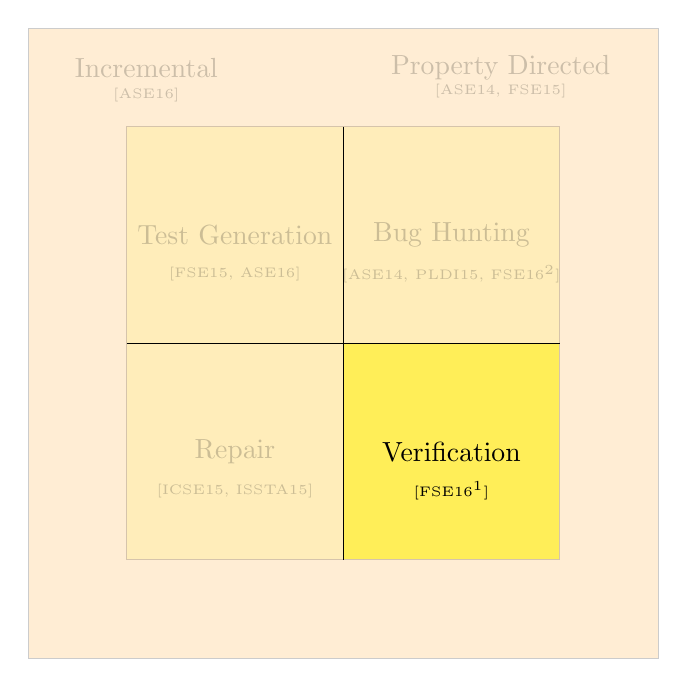
\begin{tikzpicture}
  %  \node [fill=matorange400, draw, thick, shape=rectangle, minimum width=9cm, minimum height=8cm, anchor=center] at (3cm,0) {};
  %\DrawCirc{6cm}{matyellow400}{matyellow400}{matyellow400}{matyellow400}

  \DrawSquareOpac{5.5cm}{in}
  \DrawSquareOpac{8cm}{out}
  \FillSquareOpac{out}{1}{matorange400}
  \FillSquareOpac{out}{2}{matorange400}
  \FillSquareOpac{out}{3}{matorange400}
  \FillSquareOpac{out}{4}{matorange400}

  \FillSquareOpac{in}{1}{matyellow400}
  \FillSquareOpac{in}{2}{matyellow400}
  \FillSquareOpac{in}{3}{matyellow400}
  \FillSquare{in}{4}{matyellow400}

  \DrawLines{in}


  \LabelRegionOpac{in}{1}{Test Generation}{<2->}
  \LabelRegionSmallOpac{in}{1}{[FSE15, ASE16]}{<2->}

  \LabelRegionOpac{in}{2}{Bug Hunting}{<3->}
  \LabelRegionSmallOpac{in}{2}{[ASE14, PLDI15, FSE16$^2$]}{<3->}

  \LabelRegionOpac{in}{3}{Repair}{<4->}
  \LabelRegionSmallOpac{in}{3}{[ICSE15, ISSTA15]}{<4->}

  \LabelRegion{in}{4}{Verification}{<5->}
  \LabelRegionSmall{in}{4}{[FSE16$^1$]}{<5->}


  \node[opacity=0.2] at (-2.5cm,3.5cm) {Incremental};
  \node[opacity=0.2] at (-2.5cm,3.15cm) {\tiny [ASE16]};
  \node[opacity=0.2] at (2cm,3.5cm) {Property Directed};
  \node[opacity=0.2] at (2cm,3.20cm) {\tiny [ASE14, FSE15]};

  %\node at (1.6cm,1cm) {Test Generation};
  %\node at (4.4cm,1cm) {Bug Hunting};
  %\node at (1.6cm,-1cm) {Program Repair};
  %\node at (4.4cm,-1cm) {Verification};
\end{tikzpicture}
\end{center}

\note{
  \begin{itemize}
    \item In this talk today I'lll focus on my work past work on numerical
      verification and our current unpublished directions forward
  \end{itemize}
}

\end{frame}

\section{Background}

\begin{frame}{Overview}
  \tableofcontents[currentsection,currentsubsection]
\note {
  Next, I'll give some background on nuermical abstract interpretation, and
  thread-modular analyses
}
\end{frame}

\begin{frame}[fragile]{Numerical Abstract Interpretation}
  \begin{columns}
    \begin{column}{0.6\linewidth}
      \begin{lstlisting}[name=ex01
                        , numbers=left
                        , firstnumber=1
                        , gobble=8]
        void func(int x, int y) {
          if (x >= 20) {
            y = 10;
          }
          else {
            y = 20;
          }
          assert(y > 5);
        }
      \end{lstlisting}
    \end{column}
    \begin{column}{0.4\linewidth}
        \begin{itemize}
          \item<6-> Automated proof generation
        \end{itemize}
    \end{column}
  \end{columns}
  \begin{tikzpicture}[remember picture,overlay,>=stealth']
     \draw<2->[<-,overlay] ($(pic cs:line-ex01-1-end) + (0,0)$) -| +(0.8,1.0)
     node[above,comment,thin,align=left] 
          {\normalsize 
            $x = [-\infty,\infty]$\\
            $y = [-\infty,\infty]$%
        };
     \draw<3->[<-,overlay] ($(pic cs:line-ex01-3-end) + (0,0)$) -| +(0.8,1.3)
     node[above,comment,thin,align=left] 
          {\normalsize 
            $x = [20,\infty]$\\
            $y = [10,10]$%
        };
     \draw<4->[<-,overlay] ($(pic cs:line-ex01-6-end) + (0,0)$) -| +(2.5,0.8)
     node[above,comment,thin,align=left] 
          {\normalsize 
            $x = [-\infty,19]$\\
            $y = [20,20]$%
        };
     \draw<5->[<-,overlay] ($(pic cs:line-ex01-8-end) + (0,0)$) -- +(1.8,-1.5)
     node[above,comment,thin,align=left] 
          {\normalsize 
            $x = [-\infty,\infty]$\\
            $y = [10,20]$%
        };
  \end{tikzpicture}
  \note{
    \begin{itemize}
      \item First, I'll go over numerical abstract interpretation applied to
        sequential programs
      \item As hinted by the name, the goal of numerical abstract
        interpretation is to reason about the numerical properties of a program
      \item Lets look at how a numerical analysis could be applied to this
        function
      \item First, we consider that the user of this function may pass any
        input values, so, the values of x and y are unconstrained
      \item Then, we traverse the control-flow graph of the function and update
        these inputs values for x and y based on the semantics of each
        statement
      \item So, if we enter the first branch, we know the value of x is greater
        than or equal to 20 and the value of y is updated to be 10
      \item Similarly, in the second branch, the value of x is less than 20 and
        the value of y is set to 20
      \item Finally, after exploring both branches, we join the results and get
        the fact that y is between 10 and 20 and x is unconstrained
      \item We would like to verify that at the end of the
        function the value of y is greater than 5
      \item As we can see from the results, the value of y is larger than 5 so
        we know that on all possible executions of this function the assertion
        condition will not be violated
      \item This technique allows, in general, for automated proofs such as
        this to be generated
    \end{itemize}
  }
\end{frame}

\begin{frame}[fragile,t]{Thread Modular Numerical Abstract Interpretation}
  \begin{center}
    Initially: \texttt{x = 0}
  \end{center}
  \begin{columns}
    \begin{column}{0.5\linewidth}
      \begin{lstlisting}[name=th01
                        , numbers=left
                        , firstnumber=11
                        , gobble=8]
        void thread1() {
          x = 5;
        }
      \end{lstlisting}
    \end{column}
    \begin{column}{0.5\linewidth}
      \begin{lstlisting}[name=th02
                        , numbers=left
                        , firstnumber=21
                        , gobble=8]
        void thread2() {
          int t1 = x;
          assert(x != 10);
        }
      \end{lstlisting}
    \end{column}
  \end{columns}
  \begin{center}
    \begin{itemize}
      \item<1-> Analyze threads in isolation
      \item<2-> Propagate \emph{interfering} stores to loads
      %\item<3-> Why? 
      %  \begin{itemize}
      %    \item<4-> Number of CFG nodes is exponential w.r.t.\ number of threads
      %    \item<5-> Trivially parallelized
      %  \end{itemize}
    \end{itemize}
  \end{center}
  \begin{tikzpicture}[remember picture,overlay,>=stealth']
     \draw<3->[<-,overlay] ($(pic cs:line-th01-12-end) + (0,0)$) -| +(0.8,1.0)
     node[above,comment,thin,align=left] 
          {\normalsize 
            $x = [5,5]$%
          };
     \draw<4>[<-,overlay] ($(pic cs:line-th02-22-end) + (0,0)$) -| +(0.8,1.0)
     node[above,comment,thin,align=left] 
          {\normalsize 
            $t1 = [0,0]$%
          };
     %\draw<2->[<-,overlay] ($(pic cs:line-th01-12-end) + (0,0)$) -| +(0.8,1.0)
     %node[above,comment,thin,align=left] 
     %     {\normalsize 
     %       Store on \texttt{x}
     %     };
     %\draw<3>[<-,overlay] ($(pic cs:line-th02-22-end) + (0,0)$) -| +(0.8,1.0)
     %node[above,comment,thin,align=left] 
     %     {\normalsize 
     %       Load on \texttt{x}
     %     };
     \draw<5>[<-,overlay] ($(pic cs:line-th02-22-end) + (0,0)$) -| +(0.8,1.0)
     node[above,comment,thin,align=left] 
          {\normalsize 
            $x = [0,0] \sqcup [5,5]$%
          };
     \draw<6->[<-,overlay] ($(pic cs:line-th02-22-end) + (0,0)$) -| +(0.8,1.0)
     node[above,comment,thin,align=left] 
          {\normalsize 
            $t1 = [0,5]$%
          };
  \end{tikzpicture}
  \note{
    \begin{itemize}
      \item Next, we'll look at how the previously described sequential
        analysis can be lifted to a thread-modular analysis
      \item The gist of the thread-modular numerical analysis is that each
        thread is analyzed in isolation, then, the results of the thread-local
        analysis are propagated to all other threads
      \item Consider the analysis of this two threaded program
      \item If we first analyze thread one in isolation we can see it has a
        store on the shared variable x with the value of 5
      \item Similarly, analyzing thread two, we see a shared variable read of
        x. Since the thread is analyzed in isolation, thread two can only see
        the initial value of x which is zero
      \item Then, after analyzing each thread we propagate the values stored
        into shared memory across threads 
      \item Specifically, we analyze thread two in the presense of the
        interfering store from thread one: this means thread two could either
        read the initial value or the value from thread one
      \item So, in thread two we determine the value of x to be between 0 and 5
        which is sufficient to verify that the property that x is not equal to
        10 is never violated
    \end{itemize}
  }
\end{frame}

\begin{frame}[fragile]{Issues With Prior Work}
  \begin{center}
    Initially: \texttt{x = 0}, \texttt{flag = 0}
  \end{center}
  \begin{columns}
    \begin{column}{0.5\linewidth}
      \begin{lstlisting}[name=th301
                        , numbers=left
                        , firstnumber=11
                        , gobble=8]
        void thread1() {
          x = 4;
          x = 5;
          flag = 1;
        }
      \end{lstlisting}
    \end{column}
    \begin{column}{0.5\linewidth}
      \begin{lstlisting}[name=th302
                        , numbers=left
                        , firstnumber=21
                        , gobble=8]
        void thread2() {
          int b1 = flag;
          if (b1) {
            int t1 = x;
            assert(t1 == 5);
          }
        }
      \end{lstlisting}
    \end{column}
  \end{columns}
  \begin{tikzpicture}[remember picture,overlay,>=stealth']
     \draw<2->[<-,overlay] ($(pic cs:line-th301-12-end) + (0,0)$) -| +(0.8,1.0)
     node[above,comment,thin,align=left] 
          {\normalsize 
            $x = [4,4]$%
          };
     \draw<3->[<-,overlay] ($(pic cs:line-th301-13-end) + (0,0)$) -| +(1.3,0.7)
     node[above,comment,thin,align=left] 
          {\normalsize 
            $x = [5,5]$%
          };
     \draw<3->[<-,overlay] ($(pic cs:line-th301-14-end) + (0,0)$) -| +(1.5,0.4)
     node[above,comment,thin,align=left] 
          {\normalsize 
            $\mathit{flag} = [1,1]$%
          };
     \draw<4->[<-,overlay] ($(pic cs:line-th302-22-end) + (0,0)$) -| +(1.5,0.4)
     node[above,comment,thin,align=left] 
          {\normalsize 
            $\mathit{flag} = [0,1]$%
          };
     \draw<5->[<-,overlay] ($(pic cs:line-th302-24-end) + (0,0)$) -| +(1.5,0.4)
     node[above,comment,thin,align=left] 
          {\normalsize 
            $x = [0,5]$%
          };
     \draw<6->[<-,overlay] ($(pic cs:line-th302-25-end) + (0,0)$) -| +(0.6,0.2)
     node[above,incorrect,thin,align=left] 
          {\normalsize 
            Violated!%
          };
  \end{tikzpicture}
  \begin{center}
    \begin{itemize}
      \item<1-> Interference propagation is \emph{flow-insensitive}
    \end{itemize}
  \end{center}
  \note{
    \begin{itemize}
      \item However, prior work has accuracy issues since it handles the
        propagation of values across threads in a flow-insensitive manner: we
        can see this through the following example
      \item Consider this program where thread one performs only shared memory
        writes and thread two only reads
      \item First, the assertion in thread two is never violated: in order to
        reach the assertion, flag must be true to enter the first branch, which
        means that the write of x to 5 from thread one must have already
        occurred 
      \item However, prior thread-modular analyses are unable to prove this
        condition
      \item Here's why: analyzing thread one produces three interfereces: x
        being equal to four or five, and flag being equal to true
      \item Then, analyzing thread two in the presence of these interferences
        means first that the value of flag is either zero, the initial value,
        or 1 from the interference
      \item Because flag is potentially true, we can enter the branch and
        perform the shared memory read on x
      \item Again, thread two can either read the initial value of zero or
        either 4 or 5 from thread one
      \item So, when the property is checked, we cannot show that the value of
        x must be 5: 
      \item Since this property is never actually violated in the program, this
        is a false alarm. 
    \end{itemize}
  }
\end{frame}

\begin{frame}[fragile]{Constraint-Based Abstract Interpretation}
  \begin{center}
    Initially: \texttt{x = 0}, \texttt{flag = 0}
  \end{center}
  \begin{columns}
    \begin{column}{0.5\linewidth}
      \begin{lstlisting}[name=th201
                        , numbers=left
                        , firstnumber=11
                        , gobble=8]
        void thread1() {
          x = 4;
          x = 5;
          flag = 1;
        }
      \end{lstlisting}
    \end{column}
    \begin{column}{0.5\linewidth}
      \begin{lstlisting}[name=th202
                        , numbers=left
                        , firstnumber=21
                        , gobble=8]
        void thread2() {
          int b1 = flag;
          if (b1) {
            int t1 = x;
            assert(t1 == 5);
          }
        }
      \end{lstlisting}
    \end{column}
  \end{columns}
  \only<2-3>{
    \begin{itemize}
      \item<2-> Delay the join of interferences
      \item<3-> Use constraints to prune infeasible interferences
    \end{itemize}
  }
  \only<4>{
    \begin{itemize}
      \item $(x = 4 \land \mathit{flag} = 0)$;
      \item $(x = 5 \land \mathit{flag} = 0)$;
      \item $(x = 0 \land \mathit{flag} = 0)$; 
      \item $(x = 5 \land \mathit{flag} = 1)$;
      \item $(x = 4 \land \mathit{flag} = 1)$; and
      \item $(x = 0 \land \mathit{flag} = 1)$.
    \end{itemize}
  }
  \only<5>{
    \begin{itemize}
      \item \sout{$(x = 4 \land \mathit{flag} = 0)$;}
      \item \sout{$(x = 5 \land \mathit{flag} = 0)$;}
      \item \sout{$(x = 0 \land \mathit{flag} = 0)$;}
      \item \sout{$(x = 5 \land \mathit{flag} = 1)$;}
      \item $(x = 4 \land \mathit{flag} = 1)$; and
      \item $(x = 0 \land \mathit{flag} = 1)$.
    \end{itemize}
  }
  \note{
    \begin{itemize}
      \item Our solution to this accuracy problem is two fold: first we delay
        joining together the values across all interferences, and second we use
        a system of constraints to prune infeasible interferences
      \item The combination of these two allow us to regain flow-sensitivity in
        the thread-modular analysis
      \item I'll re-analyze the previous example using our new technique to
        show both of these points
      \item First, if we consider analyzing thread two, there are six different
        combinations of interferences: x being 0, 4, or 5, and flag being
        either zero or one
      \item As we just saw, in prior work, all of these individual
        interferences would be joined together so x would be between zero and
        five, and flag would be zero or one
      \item By not joining all the values, we increase the acuraccy of the
        analysis by preventing the inclusion of spurious values
      \item Additionally, we use a system of constraints to check if all the
        possible interferences are actually feasible in the program
      \item Specifically, if we look at the six interferences, the first four
        do not violate the assertion since whenever flag is 1, x is equal to
        five
      \item For the remaining two interference combinations, our constraint
        analysis is able to show that they are infeasible in any possible
        concrete program execution
    \end{itemize}
  }
\end{frame}

\begin{frame}{Constraint Analysis}
  \begin{center}
    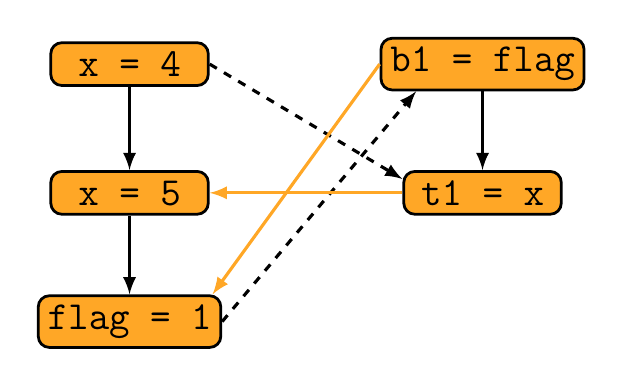
\begin{tikzpicture}
      \matrix (m) [matrix of nodes, 
        column sep=20mm,
        row sep=10mm,
        ampersand replacement=\&,
        nodes={thread},
        %nodes={draw, % General options for all nodes
        %  line width=1pt,
        %  anchor=center, 
        %  fill=matorange400,
        %  text centered,
        %  rounded corners,
        %  %minimum width=1.5cm, minimum height=8mm
        %},
          % special styles
          txt/.style={minimum width=2cm,anchor=center},
        ] {
           |[txt]| {\Large \texttt{x = 4}}       % m-1-1
           \& |[txt]| {\Large \texttt{b1 = flag}}% m-1-2
           \\
           |[txt]| {\Large \texttt{x = 5}}       % m-2-1
           \& |[txt]| {\Large \texttt{t1 = x}}   % m-2-2
           \\
           |[txt]| {\Large \texttt{flag = 1}} % m-3-1
           \& 
           \\
        };
        % decorate,decoration={snake
        %%%% MHB Arrows
        % Thread one 
        \draw<2->[-latex,garr] (m-1-1.south) -- (m-2-1.north);
        \draw<2->[-latex,garr] (m-2-1.south) -- (m-3-1.north);
        % Thread two
        \draw<2->[-latex,garr] (m-1-2.south) -- (m-2-2.north);
        %% x = 5 --> y = 5
        %\draw[-latex] (m-1-2.south) -- (m-2-2.north);
        %%%%% ReadsFrom Arrows
        % b1 reads from flag
        \draw<4->[-latex, darr] (m-3-1.east) -- ($(m-1-2.south)+ (-2.4em, 0)$);
        % t1 reads from x == 4
        \draw<3->[-latex, darr] (m-1-1.east) -- ($(m-2-2.west)+(0,0.5em)$);
        %%%%% Deduce MHB edge
        % t1 = x MHB x = 5
        \draw<5->[-latex
              , darrc
             %, decorate
             %, decoration={snake
             %             , amplitude=0.5mm
             %             , pre=lineto
             %             , pre length=12mm
             %             , post=lineto
             %             , post length=3mm}
             ]
        (m-2-2.west) -- (m-2-1.east);
        % b1 = flag MHB flag = true
        %\path ($(m-1-2.west) + (0, -0.3em)$)
        \path<6->
              (m-1-2.west)
          edge[-latex
               , darrc
              %, decorate
              %, decoration={snake
              %              , amplitude=0.5mm
              %              , pre=lineto
              %              , pre length=16mm
              %              , post=lineto
              %              , post length=1mm}
              ]
          ($(m-3-1.north) + (3em, 0)$);
        %% Infeasible reads-from edge:
        %% b = x reads from x = 5
        %\draw[-latex, dotted, red] (m-2-1.east) -- (m-1-2.west);
    \end{tikzpicture}
  \end{center}
  \begin{itemize}
    \item $(x = 4 \land \mathit{flag} = 1)$
  \end{itemize}
  \note{
    \begin{itemize}
      \item Next, I'll provide an intuition as to how our constraint analysis
        is able to determine if an interference combination is infeasible
      \vspace{-0.5em}
      \item We'll look at one of the interference combinations and show the
        constraints our analysis generates; at a high level, we use the
        program-order constraints within and across threads
      \item Again, here we have the same program with thread one on the left
        and thread two on the right
      \item The first constraints we consider are the program-order constraints
        within each thread: the execution order of statements within a thread
        must be consistent
      \item Next, we add constraints showing the flow of data across threads:
        since x reads the value of 4 from thread one, there is a flow of data
        from x equal to four to the subsequent read, and similarly for the read
        of flag
      \item Given these program-order constraints and constraints showing the
        flow of data, our analysis deduces additional implied ordering
        constraints
      \item Specifically, since the value of x is four, this means that thread
        two must have read x before thread ones subsequent write; otherwise,
        the value of x would have been overwritten
      \item Additionally, we can apply the transitive property of the ordering
        to deduce that the read of flag must have ocurred before the write
      \item Finally, if we examine the entire system of constraints, we can see
        that they form a contradiction: the read of flag must ocurr before the
        write, but also the flow of data must be from the write to the read
      \item Obviously this cannot happen, so, the interference is infeasible
    \end{itemize}
  }
\end{frame}

\section{Flow-sensitive Thread Modular Abstract Interpretation}

\begin{frame}{Overview}
  \tableofcontents[currentsection,currentsubsection]
\note {
  Now that I've gone over some examples, I'll provide the details of our new
  flow-sensitive analysis
}
\end{frame}

\begin{frame}[fragile]{Overview}
  \begin{center}
    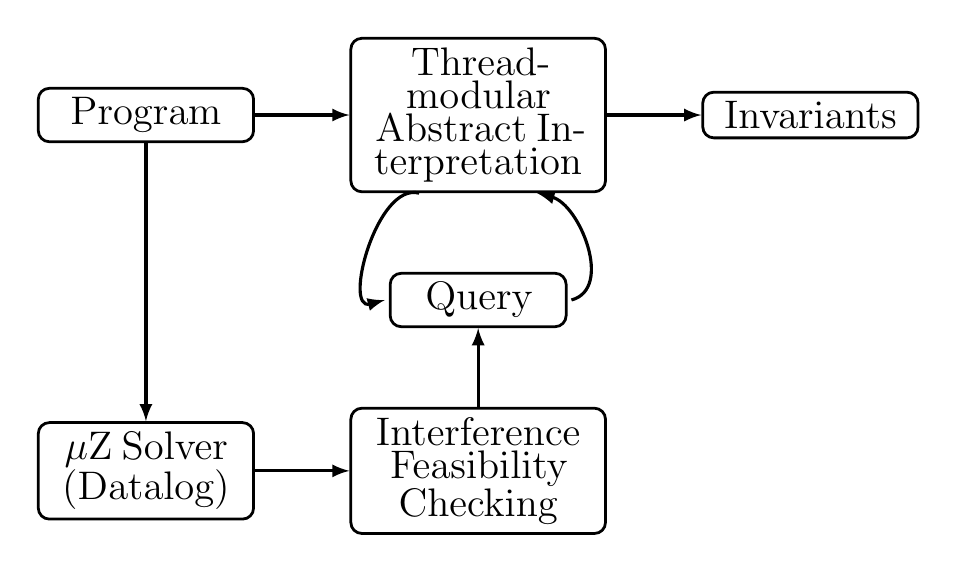
\begin{tikzpicture}
      \matrix (m) [matrix of nodes, 
        column sep=12mm,
        row sep=10mm,
        ampersand replacement=\&,
        nodes={draw, % General options for all nodes
          line width=1pt,
          anchor=center, 
          text centered,
          rounded corners,
          %minimum width=1.5cm, minimum height=8mm
        },
          % special styles
          txt/.style={minimum width=1cm,anchor=center},
        ] {
             |[txt,  text width=2.5cm]| {\Large Program}                       % m-1-1
           \& |[txt, text width=3.0cm]| {\Large Thread-modular Abstract Interpretation}    % m-1-2
           \& |[txt, text width=2.5cm]| {\Large Invariants}                             % m-1-3
           \\
           % below was previously boldfont
           \& |[txt, text width=2cm]| {\Large  Query} % m-2-2
           \&
           \\
           % below was previously boldfont
            |[txt, text width=2.5cm]|  {\Large  $\mu${Z} Solver (Datalog)}      % m-3-1
           % below was previously boldfont
           \& |[txt, text width=3.0cm]| {\Large  Interference Feasibility Checking} % m-3-2
           \\
     }; % end matrix
      \draw[-latex,garr] (m-1-1.east) -- (m-1-2.west);
      \draw[-latex,garr] (m-1-2.east) -- (m-1-3.west);

      \draw[-latex,garr] ([xshift=0.05cm]m-2-2.east) to [out=15,in=-15]  ([xshift=0.75cm]m-1-2.south);
      \draw[-latex,garr] ([xshift=-0.75cm]m-1-2.south) to [out=165,in=195]  ([xshift=-0.05cm]m-2-2.west);
   
      \draw[-latex,garr] (m-1-1.south) -- (m-3-1.north);
      \draw[-latex,garr] (m-3-1.east) -- (m-3-2.west);
      \draw[-latex,garr] (m-3-2.north) -- (m-2-2.south);
    \end{tikzpicture}
  \end{center}
  \note{
    \begin{itemize}
      \item Here is a high-level overview of our new method
      \item We start with an input program we'd like to analyze
      \item We first perform an analysis to generate a set of constraints from
        the program which are fed into our constraint solver, which is a
        datalog solver
      \item Then, we perform a thread-modular analysis of each thread in the
        program
      \item During the thread modular analysis, as I just showed, each
        interference combination is analyzed in isolation
      \item Additionally, the abstract interpreter queries the solver to check
        if a certain interference combination is actually feasible
      \item If it is feasible, then it is analyzed, while if it is determined
        infeasible the interference can be safely skipped
      \item The end result is that each location in the program is annotated
        with a set of numerical invariants 
      \item These invariants can then be used for things like property
        verification
    \end{itemize}
  }
\end{frame}

\begin{frame}[fragile]{Flow-sensitive Thread-modular Abstract Interpretation}
  %\begin{center}
  %  Initially: \texttt{x = 0}, \texttt{flag = 0}
  %\end{center}
  \begin{columns}
    \begin{column}{0.5\linewidth}
      \begin{lstlisting}[name=th201
                        , numbers=left
                        , firstnumber=11
                        , gobble=8]
        void thread1() {
          x = 4;
          x = 5;
          flag = 1;
        }
      \end{lstlisting}
    \end{column}
    \begin{column}{0.5\linewidth}
      \begin{lstlisting}[name=th202
                        , numbers=left
                        , firstnumber=21
                        , gobble=8]
        void thread2() {
          int b1 = flag;
          if (b1) {
            int t1 = x;
            assert(t1 == 5);
          }
        }
      \end{lstlisting}
    \end{column}
  \end{columns}
  \only<1-7>{
    \begin{itemize}[<+->]
      \item Interferences from thread one:
        \begin{itemize}
          \item $s_{x_1}: \texttt{x = 4}$
          \item $s_{x_2}: \texttt{x = 5}$
          \item $s_{f}: \texttt{flag = 1}$
        \end{itemize}
      \item Loads from thread two:
        \begin{itemize}
          \item $l_f$
          \item $l_x$
        \end{itemize}
    \end{itemize}
  } %only
  \only<8>{
    \begin{itemize}
      \item Store-load-pairs: $(l_x, \Set{s_{x_1}, s_{x_2}})
                               , (l_f, \Set{s_{f}})
                              $
    \end{itemize}
  }
  \begin{itemize}
    \item<9-> Load-store-pairs: $(l_x, \Set{s_{x_1}, s_{x_2}, s_d})
                             , (l_f, \Set{s_{f}, s_d})
                            $
    \item<10-> Interference Combinations:
      \begin{itemize}[<+->]
        \item $(\langle l_x, s_{x_1} \rangle
               , \langle l_f, s_{f} \rangle
               )$
        \item $(\langle l_x, s_{x_1} \rangle
               , \langle l_f, s_{d} \rangle
               )$
        \item $(\langle l_x, s_{x_2} \rangle
               , \langle l_f, s_{f} \rangle
               )$
        \item $(\langle l_x, s_{x_2} \rangle
               , \langle l_f, s_{d} \rangle
               )$
        \item $(\langle l_x, s_{d} \rangle
               , \langle l_f, s_{f} \rangle
               )$
        \item $(\langle l_x, s_{d} \rangle
               , \langle l_f, s_{d} \rangle
               )$
      \end{itemize}
  \end{itemize}
  \note{
    \begin{itemize}
      \item Next, we'll look into closer detail of our flow-sensitive and
        thread-modular abstract interpretation; to do so, we'll again look at
        the same running example
      \item The gist of our technique is to explicitly test the cartesian
        product of all feasible store-to-load interferences
      \item First, we can see there are three interfering stores from thread
        one: two on x, setting it to four and give, and one on flag
      \item Similarly, there are two loads in thread two: one on flag and
        another on x
      \item Next, we pair each each load with every store to the same variable.
        This explicitly shows all the possible inter-thread data flows
      \item In addition to this, we have to consider the thread not reading
        from values from other threads but also reading values from itself. To
        this end, we use a special store $s_d$ to represent the thread reading
        from its own local memory
      \item Next, we take the Cartesian product of all these sets which
        enumerates all the possible pairings of every load to a single store:
        these are the six possible combinations we looked at in the previous
        example
      \item Given these each of these combinations, we next check if each one
        individually is feasible in the program
    \end{itemize}
  }
\end{frame}

\begin{frame}{Checking Interference Feasibility}
  \begin{itemize}[<+->]
    \item Horn-clauses with finite domains 
      \begin{itemize} 
        \item Solved in polynomial time
      \end{itemize}
    \item Must-happen-before relation
      \begin{itemize}
        \item Only analyze a single interference combination
      \end{itemize}
    \item Contradictions in must-happen-before indicate infeasibility
    \item Sound
      \begin{itemize}
        \item Under-approximate must-happen-before
      \end{itemize}
  \end{itemize}
  \note{
    \begin{itemize}
      \item To check the feasibility of interferences, we generate and check
        the feasibility of a set of horn clauses over finite domains
      \item We used horn-clauses, as opposed to other constraints like SMT or
        SAT, because they have efficient decision procedures: satisfiability
        can be checked in polynomial time
      \item The main goal of our analysis is to determine which store-to-load
        flows are infeasible; we do this mostly by generating the
        must-happen-before relation; this relation indicates that two
        statements must have a specific ordering
      \item One of the keys to making our analysis accurate is that we only
        generate the must-happen-before relation with respect to a single
        interference combination as opposed to over the entire program
      \item Finally, we also ensure our constraint analysis is sound: to do
        this, we ensure that we under-approximate the must-happen-before
        relation
      \item This means that whenever we determine an interference combination
        as infeasible, it definitely is infeasible in the actual program
      \item However, we do not guarantee that all infeasible interference
        combinations will be detected
    \end{itemize}
  }
\end{frame}

\begin{frame}{Deduction Rules}
  \begin{center}
    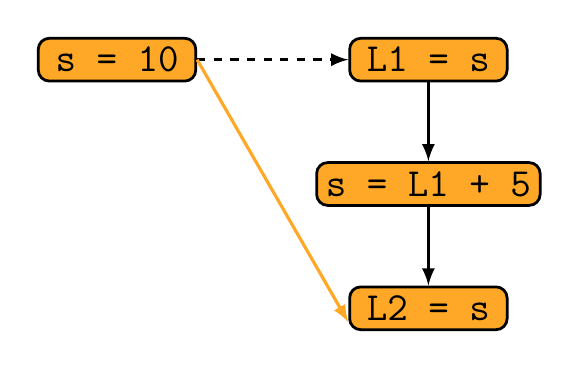
\begin{tikzpicture}
      \matrix (m) [matrix of nodes, 
        column sep=15mm,
        row sep=10mm,
        ampersand replacement=\&,
        nodes={thread},
        %nodes={draw, % General options for all nodes
        %  line width=1pt,
        %  anchor=center, 
        %  text centered,
        %  rounded corners,
        %  %minimum width=1.5cm, minimum height=8mm
        %},
          % special styles
          txt/.style={minimum width=2cm,anchor=center},
        ] {
           |[txt]| {\Large \texttt{s = 10}}       % m-1-1
           \& |[txt]| {\Large \texttt{L1 = s}}       % m-1-2
           \\
           \& |[txt]| {\Large \texttt{s = L1 + 5}}     % m-2-2
           \\
           \& |[txt]| {\Large \texttt{L2 = s}}     % m-3-2
           \\
        };
        %%%%% MHB Arrows
        %% l1 = s --> s + t + 5
        \draw<1->[garr,-latex] (m-1-2.south) -- (m-2-2.north);
        %% s + t + 5 -> l1 = s
        \draw<1->[garr,-latex] (m-2-2.south) -- (m-3-2.north);
        %% ReadFrom edges
        % l1 = s <-- s = 10
        \draw<2->[garr,-latex, dashed] (m-1-1.east) -- (m-1-2.west);
        %% Infeasible reads-from edge:
        % l2 = s --> s = 10
        \draw<3->[-latex, darrc] (m-1-1.east) -- ($(m-3-2.west)+(0em,-0.5em)$);
    \end{tikzpicture}
  \end{center}
  \note{
    \begin{itemize}
      \item We created a bunch of deduction rules capturing various scenarios
        where a must-happen-before edge can be inferred 
      \item Here's an example of one of them. We have one thread on the left
        performing a store, and a thread on the right performing a load, store,
        and the subsequent load
      \item The program-order constraints within each thread are represented by
        the black arrows
      \item Suppose that the interference combination we are analyzing contains
        a store-to-load flow as shown by the dashed edge
      \item Notice that the right thread is first performing a shared memory
        read and then performing a shared memory write on the same variable
      \item This means that the subsequent memory read cannot read the same
        value: this is because the thread has already overwritten it
      \item So, we deduce that given the first store-to-load flow, the second
        yellow store-to-load flow of the right thread is infeasible
      \item This means that any interference combination containing this
        infeasible store-to-load combination can be removed from the analysis
      \item We created other deduction rules in a similar fashion by examining
        other situations where inter-thread flows become infeasible
    \end{itemize}
  }
\end{frame}


\begin{frame}{Optimizations}
  \begin{itemize}[<+->]
    \item Property directed pruning
    \item Clustering
  \end{itemize}
  \note{
    %\begin{itemize}
    %  \item Next, I'll go over two optimizations we created for our technique
    %  \item The two optimizations we used we call property directed pruning and
    %    clustering
    %\end{itemize}
    \begin{itemize}
      \item We introduced two optimizations, one making the analysis property
        directed, and another we called clustering
      \item Clustering groups together loads and stores into subsets and only
        explores the combinations within these clusters, similar to the packing
        of relational abstract domains
      \item For the sake of time, I wont go into these details
    \end{itemize}
  }
\end{frame}

\begin{frame}[fragile]{Overview}
  \begin{center}
    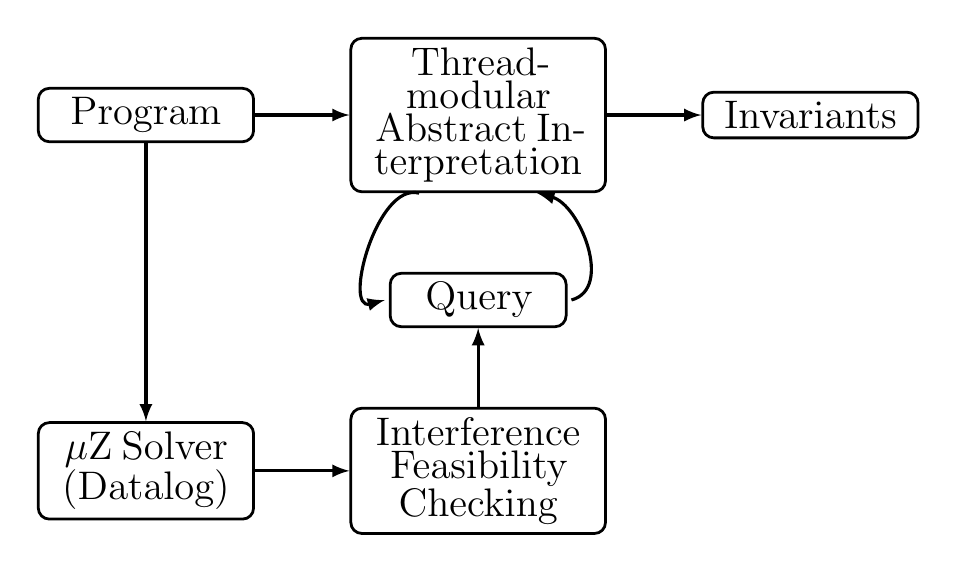
\begin{tikzpicture}
      \matrix (m) [matrix of nodes, 
        column sep=12mm,
        row sep=10mm,
        ampersand replacement=\&,
        nodes={draw, % General options for all nodes
          line width=1pt,
          anchor=center, 
          text centered,
          rounded corners,
          %minimum width=1.5cm, minimum height=8mm
        },
          % special styles
          txt/.style={minimum width=1cm,anchor=center},
        ] {
             |[txt,  text width=2.5cm]| {\Large Program}                       % m-1-1
           \& |[txt, text width=3.0cm]| {\Large Thread-modular Abstract Interpretation}    % m-1-2
           \& |[txt, text width=2.5cm]| {\Large Invariants}                             % m-1-3
           \\
           % below was previously boldfont
           \& |[txt, text width=2cm]| {\Large  Query} % m-2-2
           \&
           \\
           % below was previously boldfont
            |[txt, text width=2.5cm]|  {\Large  $\mu${Z} Solver (Datalog)}      % m-3-1
           % below was previously boldfont
           \& |[txt, text width=3.0cm]| {\Large  Interference Feasibility Checking} % m-3-2
           \\
     }; % end matrix
      \draw[-latex,garr] (m-1-1.east) -- (m-1-2.west);
      \draw[-latex,garr] (m-1-2.east) -- (m-1-3.west);

      \draw[-latex,garr] ([xshift=0.05cm]m-2-2.east) to [out=15,in=-15]  ([xshift=0.75cm]m-1-2.south);
      \draw[-latex,garr] ([xshift=-0.75cm]m-1-2.south) to [out=165,in=195]  ([xshift=-0.05cm]m-2-2.west);
   
      \draw[-latex,garr] (m-1-1.south) -- (m-3-1.north);
      \draw[-latex,garr] (m-3-1.east) -- (m-3-2.west);
      \draw[-latex,garr] (m-3-2.north) -- (m-2-2.south);
    \end{tikzpicture}
  \end{center}
  \note{
    \begin{itemize}
      \item At this point, I've gone over all the big points of our
        flow-sensitive analysis
      \item I first showed how we considered and calculated different
        interference combinations during the thread-modular abstract
        interpretation
      \item And second, I showed some examples of how we determine if certain
        interference combinations were infeasible
      \item By repeatedly applying these two steps, we generate a set of more
        accurate invariants, compared to prior work, for each thread
    \end{itemize}
  }
\end{frame}

\section{Extensions}


\begin{frame}{Overview}
  \tableofcontents[currentsection]
\note {
  Next, I'll go over two extensions to the prior constraint-based analysis:
  handling weak-memory, and making the analysis incremental
}
\end{frame}

\subsection{Weak Memory}
\begin{frame}{Handling to TSO/PSO/RMO}
  \begin{center}
    Initially: \texttt{x = flag = 0}
    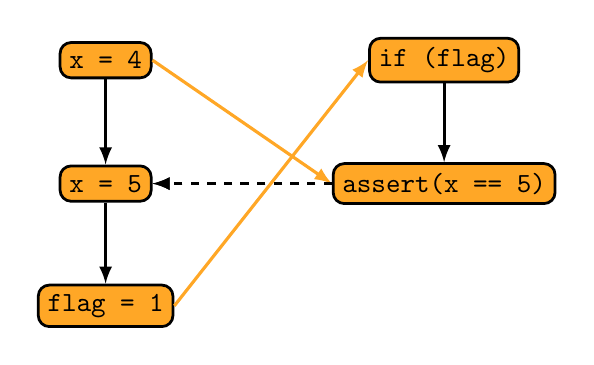
\begin{tikzpicture}
      \matrix (wm) [matrix of nodes
                    , column sep=20mm
                    , row sep=10mm
                    % Beamer messes with everything
                    , ampersand replacement=\&
                   ]
       {
         |[thread]| {\texttt{x = 4}} 
         \& |[thread]|{\texttt{if (flag)}} 
         \\
         |[thread]|{\texttt{x = 5}} 
         \& |[thread]|{\texttt{assert(x == 5)}}
         \\
         |[thread]|{\texttt{flag = 1}} 
         \& {}
         \\
       };%matrix
       \draw[>=latex,->, garr] (wm-1-1.south) -- (wm-2-1.north);
       \draw[>=latex,->, garr, visible on=<1-3>] (wm-2-1.south) -- (wm-3-1.north);
       \draw[>=latex,->, garr] (wm-1-2.south) -- (wm-2-2.north);

       \draw[>=latex,->, darrc, visible on=<2->] (wm-1-1.east) -- (wm-2-2.west);
       \draw[>=latex,->, darrc, visible on=<2->] (wm-3-1.east) -- (wm-1-2.west);
       \draw[>=latex,->, darr, visible on=<3->] (wm-2-2.west) -- (wm-2-1.east);
       % This duplicate arrow is necessary to get the 4th slide to appea, and
       % thus make the arrow between (2,1) and (3,1) disappear after the third
       % slide. 
       \draw[>=latex,->, darr, visible on=<4->] (wm-2-2.west) -- (wm-2-1.east);
    \end{tikzpicture}
  \end{center}
  \note{
    \begin{itemize}
      \item The previous constraint analysis reasoning about interference
        infeasibility assumed sequential consistency 
      \item Sequential consistency was assumed since program-order constraints
        between statements were used in the analysis not necessarily enforced
        under certain weak memory models
      \item For example, consider this program where the left thread sets x to
        4, and then to 5, and then sets flag to 1
      \item The right thread checks if the value of flag is one, and, if so,
        asserts that x is 5
      \item Consider the case where the right thread reads flag to be 1, and
        x to be 4
      \item Under SC this exection is safe since in order for x to be 4 the
        assertion must execute before the second write to x, which means flag
        cannot be one
      \item But, under PSO and RMO, writes to different variables may be
        reordered, so, conceptually, the write to flag may occur before the
        writes to x
      \item To compensate for this, we developed a set of new inference rules
        sound under TSO, PSO, and RMO
    \end{itemize}
  }
\end{frame}

\subsection{Incremental Analysis}

\begin{frame}[c]{Incremental Analysis}
  \begin{itemize}[<+->]
    \item Given previously analyzed prgoram $P_1$ analyze new version $P_2$
    \item Ignore unimpacted regions 
    \item Reuse old analysis information
  \end{itemize}
  \note{
    \begin{itemize}
      \item Next I'll show how we made out constraint-based thread-modular
        analyzer incremental
      \item The gist of an incremental analysis is given an old program version
        which was previously analyzed, analyze a new program version
      \item This provides an decrease in runtime overhead since the analysis
        can ignore regions unimpacted by the modifications
      \item Also, analysis results from the old version can be reused and
        passed to the new version
    \end{itemize}
  }
\end{frame}

\begin{frame}[fragile]{Change-Impact Analysis}
  \begin{columns}[c]
    \begin{column}{0.5\textwidth}
      \begin{lstlisting}[name=ci01
                        , numbers=left
                        , firstnumber=1
                        , gobble=8]
        x = func();
        y = otherFunc();
        if (!x) {
          x = -1;
        }
        if (!y) {
          y = -1;
        }
      \end{lstlisting}
    \end{column}
    \begin{column}{0.5\textwidth}
      \begin{lstlisting}[name=ci01
                        , numbers=left
                        , firstnumber=1
                        , gobble=8]
        x = (*\textcolor{matred400}{coolFunc();}*)
        y = otherFunc();
        if (!x) {
          x = -1;
        }
        if (!y) {
          y = -1;
        }
      \end{lstlisting}
    \end{column}
  \end{columns}
  \note{
    \begin{itemize}
      \item Identifying regions impacted by code modifications is done by
        what's called a change-impact analysis
      \item Here, we take modifications to the old program, and identify
        regions in the new program which may be impacted by the change 
      \item Suppose the first function called was changed from func to coolFunc
      \item What we would like to know are the other statements in the program
        impacted by this modifications
    \end{itemize}
  }
\end{frame}

\begin{frame}{Change-Impact Analysis}
  \begin{center}
    \only<1>{
    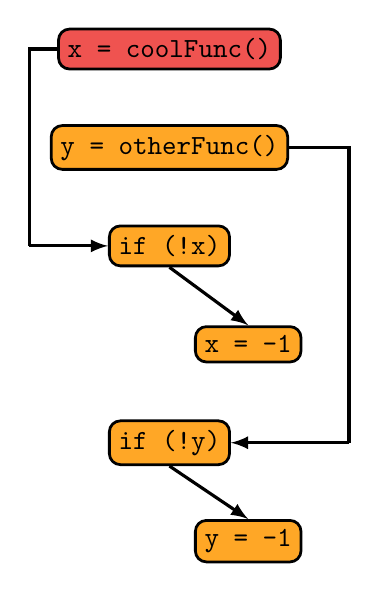
\begin{tikzpicture}[node distance=1.25cm]
      \node[thread,fill=matred400] (xf) {\texttt{x = coolFunc()}};
      \node[thread, below of=xf] (yf) {\texttt{y = otherFunc()}};
      \node[thread, below of=yf] (ifx) {\texttt{if (!x)}};
      \node[thread, below of=ifx, xshift=1.0cm] (xeq) {\texttt{x = -1}};
      \node[thread, below of=xeq, xshift=-1.0cm] (ify) {\texttt{if (!y)}};
      \node[thread, below of=ify, xshift=1.0cm] (yeq) {\texttt{y = -1}};

      \draw[garr] (xf.west) -| ([xshift=-1.0cm]ifx.west);
      \draw[garr,>=latex,->] ([xshift=-1.0cm]ifx.west) -- (ifx.west);

      \draw[garr] (yf.east) -| ([xshift=1.5cm]ify.east);
      \draw[garr,>=latex,->] ([xshift=1.5cm]ify.east) -- (ify.east);

      \draw[garr,>=latex,->] (ifx.south) -- (xeq.north);

      \draw[garr,>=latex,->] (ify.south) -- (yeq.north);
    \end{tikzpicture}
  }%only<1>
    \only<2->{
    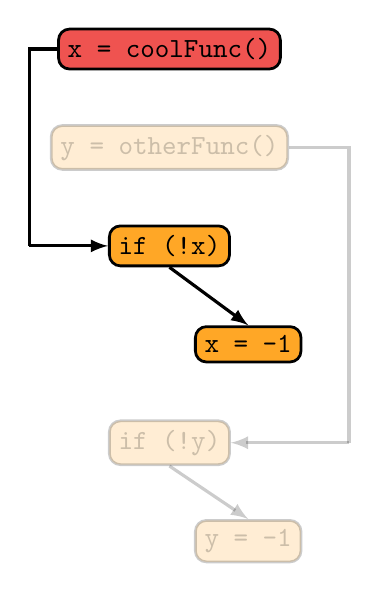
\begin{tikzpicture}[node distance=1.25cm]
      \node[thread,fill=matred400] (xf) {\texttt{x = coolFunc()}};
      \node[opacity=0.2,thread, below of=xf] (yf) {\texttt{y = otherFunc()}};
      \node[thread, below of=yf] (ifx) {\texttt{if (!x)}};
      \node[thread, below of=ifx, xshift=1.0cm] (xeq) {\texttt{x = -1}};
      \node[opacity=0.2,thread, below of=xeq, xshift=-1.0cm] (ify) {\texttt{if (!y)}};
      \node[opacity=0.2,thread, below of=ify, xshift=1.0cm] (yeq) {\texttt{y = -1}};

      \draw[garr] (xf.west) -| ([xshift=-1.0cm]ifx.west);
      \draw[garr,>=latex,->] ([xshift=-1.0cm]ifx.west) -- (ifx.west);

      \draw[opacity=0.2,garr] (yf.east) -| ([xshift=1.5cm]ify.east);
      \draw[opacity=0.2,garr,>=latex,->] ([xshift=1.5cm]ify.east) -- (ify.east);

      \draw[garr,>=latex,->] (ifx.south) -- (xeq.north);

      \draw[opacity=0.2,garr,>=latex,->] (ify.south) -- (yeq.north);
    \end{tikzpicture}
  }%only<1->
  \end{center}
  \note{
    \begin{itemize}
      \item To do this, we first build the program dependency graph, and then
        compute all the statements reachable from the modified statement
      \item Specifically, this graph shows both the data and control
        dependencies between statements
      \item The statements reachable in the graph from the modified statements
        are only those involving x
      \item Now we can start to see why a change-impact analysis is useful to
        couple with an analyzer: it can automatically reduce the number of
        statements of interest
    \end{itemize}
  }
\end{frame}



\begin{frame}[fragile]{Change-Impact Analysis for Weak Memory}

\begin{columns}[c]
\begin{column}{0.5\textwidth}
\begin{lstlisting}[language=C]
x = y = z = 0;
flag1 = flag2 = 0;
void thread1() { 
  x = 5;
  y = 10;
  fence;
  flag1 = 1;
}
void thread2() { 
  z = 1;
  fence;
  flag2 = 1;
}
void thread3() {
  if (flag1)
    assert(x + y == 15);
  if (flag2)
    assert(z == 1);
}
\end{lstlisting}
\end{column}
\begin{column}{0.5\textwidth}
  \begin{onlyenv}<2->
\begin{lstlisting}[language=C]
x = y = z = 0;
flag1 = flag2 = 0;
void thread1() { 
  x = 5;
  y = 10;
  (*\textcolor{red}{SSMembar;}*)
  flag1 = 1;
}
void thread2() { 
  z = 1;
  fence;
  flag2 = 1;
}
void thread3() {
  if (flag1)
    assert(x + y == 15);
  if (flag2)
    assert(z == 1);
}
\end{lstlisting}%
\end{onlyenv}%
\end{column}
\end{columns}
  \note{
    \begin{itemize}
      \item But, to the best of our knowledge no such change-impact analysis,
        or dependency analysis, exists handling weak-memory, particularly the
        weak-memory related statements such as fences and memory barriers
      \item For example, consider this program where threads 1 and 2
        synchronize with thread 3 using flag1 and flag2, respecitively.
      \item Thread one updates the values of x and y and then sets flag1 to
        true, and thread two updates the value of z and then sets flag2 to true
      \item Thread 3 reads the value of x and y only if flag1 is set, and
        similarly reads z only if flag2 is set
      \item Suppose the fence in thread one is modified to a store-store memory
        barrier, that is, a synchronization operation ensuring all stores
        before the barrier have flushed to memory before any subsequent
        operation
      \item We would like to know the impacted statements in the program from
        this change, and to do this we need the dependency graph
    \end{itemize}
  }
\end{frame}

\begin{frame}{Weak-Memory Dependency Analysis}
%\begin{adjustbox}{totalheight=\textheight-2\baselineskip}
  \begin{center}
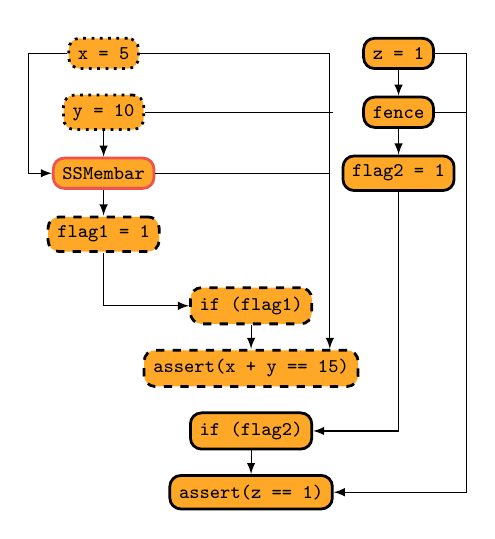
\begin{tikzpicture}
  \tikzstyle{node}=[thread,font=\scriptsize]
  %\tikzstyle{node}=[draw
  %                  , fill=matorange400
  %                  , line width=1pt
  %                  , anchor=center
  %                  , text centered
  %                  , rounded corners
  %                  , font=\scriptsize]
  \tikzstyle{imp}=[thread, dashed, font=\scriptsize]
  %\tikzstyle{imp}=[draw
  %                 , line width=1pt
  %                 , ggreen
  %                 , anchor=center
  %                 , text centered
  %                 , dashed
  %                 , rounded corners
  %                 , font=\scriptsize]
  \tikzstyle{may-imp}=[node, dotted]
  \tikzstyle{mod}=[node, draw=matred400, rectangle]
\matrix (m) [
 matrix of nodes
 , column sep=23mm
 , row sep=3mm
, ampersand replacement=\&
]{
  \node [may-imp,align=center] (x5) { \texttt{x = 5}};
  \& \node [node,align=center] (z1) { \texttt{z = 1}}; \\
%
  \node [may-imp,align=center] (y10) { \texttt{y = 10}};
  \& \node [node,align=center] (fright) { \texttt{fence}}; \\
%
  \node [mod,align=center] (fleft) { \texttt{SSMembar}};
  \& \node [node,align=center] (fl2) { \texttt{flag2 = 1}}; \\
%
  \node [imp,align=center] (fl1) { \texttt{flag1 = 1}};
  \&  \\
};%end matrix
  \node [imp,align=center,below=3mm of m] (if-f1) {\texttt{if (flag1)}};
  \node [imp,align=center,below=3mm of if-f1] (as1) {\texttt{assert(x + y == 15)}};
  \node [node,align=center,below=3mm of as1] (if-f2) {\texttt{if (flag2)}};
  \node [node,align=center,below=3mm of if-f2] (as2) {\texttt{assert(z == 1)}};

  \draw [-latex] (x5.east) -| ([xshift=10mm]as1.north);

  \draw  (x5.west) -| ([xshift=-3mm]fleft.west);
  \draw [-latex] ([xshift=-3mm]fleft.west) -- (fleft.west);

  \draw [-latex] (y10.south) -- (fleft.north);
  \draw [-latex] (fleft.south) -- (fl1.north);

  \draw [-latex] (fl1.south) |- (if-f1.west);
  
  \draw [-latex] (z1) -- (fright);
  \draw [-latex] (fright) -- (fl2);

  \draw [-latex] (fl2) |- (if-f2);

  \draw [-latex] ([xshift=4mm]fright.east) |- (as2.east);
  \draw (fright.east) -- ([xshift=4mm]fright.east);

  \draw ([xshift=4mm] z1.east) -- ([xshift=4mm]fright.east);
  \draw (z1.east) -- ([xshift=4mm] z1.east);
  
  \draw (y10.east) -- ([xshift=23.8mm]y10.east);
  \draw (fleft.east) -- ([xshift=22.2mm]fleft.east);

  \draw [-latex] (if-f1) -- (as1);
  \draw [-latex] (if-f2) -- (as2);

\end{tikzpicture}
%\end{adjustbox}
\end{center}
\note{
  \begin{itemize}
    \item To reason about dependencies involving weak-memory primitives we use
      what we call a semi flow-insensitive analysis: we perform the dependency
      analysis in a flow insensitive way except for with regards to fences and
      memory barriers
    \item Semantically, we consider a fence to be a flush of the store-buffers
      of a thread, so, it acts as a write to all variables ocurring before the
      fence
    \item To ensure soundness, some other peculiarties have to be delt with but
    \item For the sake of time, I wont go into the details but if you're
      interested I'd be happy to offline
    \item But, given the weak-memory aware dependency analysis we are able to
      formulate a change-impact analysis sound under weak-memory
  \end{itemize}
}
\end{frame}

\begin{frame}{Incremental Thread-Modular Analysis}
  \begin{itemize}[<+->]
    \item May be impacted
    \item May impact
    \item Preserve analysis results
    \item Ignore transfer functions
  \end{itemize}
  \note{
    \begin{itemize} 
      \item Very briefly, I'll go over how we created an incremental
        thread-modular analyzer
      \item We make use of two types of impact information: the first, as we
        saw before, are identifying statements in the program which may-be
        impacted by the change
      \item The second, are statements which may-impact impacted statements
      \item Using this information we are able to preserve analysis results
        from the old program version, as well as ignore the transfer functions
        of many statements
      \item This causes the analysis to converge much faster and thus reduce
        runtime
    \end{itemize} 
  } 
\end{frame}


\section{Experiments}

\begin{frame}{Overview}
  \tableofcontents[currentsection,currentsubsection]
\note {
  Next I'll summarize our experimental results. All tests were done on a
  consumer linux laptop with 8 GB of ram and a 2.8 GHz x86 processor
}
\end{frame}

\begin{frame}{Constraint-Based Abstract Interpreter for SC}
  \begin{itemize}[<+->]
    \item 38 C programs (SVComp, device drivers)
    \item Compared to Min\`{e} [VMCAI 2014]
      \begin{itemize}
        \item 38 verified properties
        \item 154s runtime
      \end{itemize}
    \item Our fully optimized approach 
      \begin{itemize}
        \item 1,078 verified properties
        \item 480s runtime
      \end{itemize}
    \item 28x more verified properties
    \item 3x increase in time
  \end{itemize}
  \note{
    \begin{itemize}
      \item First, here are the results of our tool testing sequentially
        consistent programs.
      \item We ran our tool on 38 C programs and compared it against Mine's
        non-constraint based thread-modular analyzer
      \item His approach was able to verify 38 properties in 154 seconds,
        whereas our tool verified 1,078 properties in 480 seconds
      \item This is a total of 28 more verified properties with a 3x increase
        in runtime
    \end{itemize}
  }
\end{frame}

\begin{frame}{Constraint-Based Abstract Interpreter for TSO, PSO, and RMO}
  \begin{itemize}[<+->]
    \item 52 C programs (device drivers), litmus tests
    \item Compared to Min\`{e}
      \begin{itemize}
        \item 1752 verified properties
        \item 415s
      \end{itemize}
    \item Compared to Duet [Farzan and Kincaid, POPL 2012]
      \begin{itemize}
        \item 2432 verified properties
        \item 106s
      \end{itemize}
    \item Our new method
      \begin{itemize}
        \item 4577 verified properties
        \item 5387s
      \end{itemize}
    \item 12--50x runtime increase
    \item 1.8--2.6x increase in verified properties
  \end{itemize}
  \note{
    \begin{itemize}
      \item Next, we evaluated our approach sound under TSO, PSO and RMO
      \item We again compared against Mine, and also a tool by Farzan and
        Kincaid called Duet
      \item We tested on 52 C programs as well as a large selection of Litmus
        tests
      \item Mine was able to verify 1752 properties in 415 seconds, Duet 2432
        properties in 106 seconds, and our tool verified 4577 properties in
        5387 seconds
      \item This is a 12--50x increase in runtime for a 1.8--2.6x increase in
        the number of verified properties
    \end{itemize}
  }
\end{frame}

\begin{frame}{Incremental Constraint-Based Abstract Interpreter for TSO, PSO, and RMO}
  \begin{itemize}[<+->]
      \item Average 57\% of program impacted by modifications
      \item Ranging from 1.5\%--92\%
      \item Min\'{e}
        \begin{itemize}
          \item 6384 verified properties
          \item 1263 seconds
        \end{itemize}
      \item Incremental w/o constraints
        \begin{itemize}
          \item 6384 verified properties
          \item 748 seconds
        \end{itemize}
      \item Non-incremental with constraints
        \begin{itemize}
          \item 11,463 verified properties
          \item 14,389 seconds
        \end{itemize}
      \item Incremental with constraints
        \begin{itemize}
          \item 11,463 verified properties
          \item 2642 seconds
        \end{itemize}
    \end{itemize}
  \note{
    \begin{itemize}
      \item Finally, here are the results for our incremental analyzer. We
        compared again to Min\'{e} and implemented an incremental version of
        both his algorithm, as well as our constaint-based analyzer
      \item Our test set had 57\% of the program impacted on average, ranging
        from 1.5 to 92 percent.
      \item First, his approach verified 6384 properties in 1,263 seconds,
        whereas our incremental version verified the same number of properties
        in 748 seconds, about a 1.7x speedup
      \item Second, the constraint based approach took 14,000 seconds to verify
        11,458 properties, whereas our incremental version took only 2642
        seconds to verify the same number of properties, about a 5.4x speedup
    \end{itemize}
  }
\end{frame}

\begin{frame}{Conclusion}
  \begin{itemize}[<+->]
    \item Constraint-Based Thread-Modular Abstract Interpretation
    \item Handling TSO, PSO, RMO
    \item Weak-memory aware change-impact analysis
    \item Incremental thread-modular abstract interpretation
  \end{itemize}
  \note{
    \begin{itemize}
      \item So, in conclusion I presented a constraint-based thread-modular
        abstract interpretation algorithm
      \item I introduced how it can be extended to handle TSO, PSO, and RMO
      \item Also, I showed the intuition behind a weak-memory aware
        change-impact analysis, and a incremental thread-modular analyzer
    \end{itemize}
  }
\end{frame}

\begin{frame}

\begin{center}
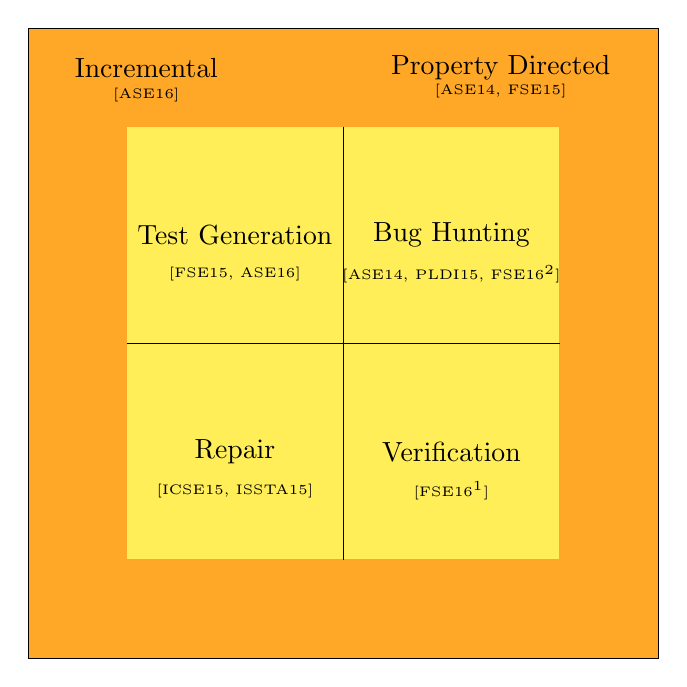
\begin{tikzpicture}
  %  \node [fill=matorange400, draw, thick, shape=rectangle, minimum width=9cm, minimum height=8cm, anchor=center] at (3cm,0) {};
  %\DrawCirc{6cm}{matyellow400}{matyellow400}{matyellow400}{matyellow400}

  \DrawSquare{5.5cm}{in}
  \DrawSquare{8cm}{out}
  \FillSquare{out}{1}{matorange400}
  \FillSquare{out}{2}{matorange400}
  \FillSquare{out}{3}{matorange400}
  \FillSquare{out}{4}{matorange400}

  \FillSquare{in}{1}{matyellow400}
  \FillSquare{in}{2}{matyellow400}
  \FillSquare{in}{3}{matyellow400}
  \FillSquare{in}{4}{matyellow400}

  \DrawLines{in}


  \LabelRegionVis{in}{1}{Test Generation}{<2->}
  \LabelRegionSmallVis{in}{1}{[FSE15, ASE16]}{<2->}

  \LabelRegionVis{in}{2}{Bug Hunting}{<3->}
  \LabelRegionSmallVis{in}{2}{[ASE14, PLDI15, FSE16$^2$]}{<3->}

  \LabelRegionVis{in}{3}{Repair}{<4->}
  \LabelRegionSmallVis{in}{3}{[ICSE15, ISSTA15]}{<4->}

  \LabelRegionVis{in}{4}{Verification}{<5->}
  \LabelRegionSmallVis{in}{4}{[FSE16$^1$]}{<5->}


  \node[visible on=<6->] at (-2.5cm,3.5cm) {Incremental};
  \node[visible on=<6->] at (-2.5cm,3.15cm) {\tiny [ASE16]};
  \node[visible on=<7->] at (2cm,3.5cm) {Property Directed};
  \node[visible on=<7->] at (2cm,3.20cm) {\tiny [ASE14, FSE15]};

  %\node at (1.6cm,1cm) {Test Generation};
  %\node at (4.4cm,1cm) {Bug Hunting};
  %\node at (1.6cm,-1cm) {Program Repair};
  %\node at (4.4cm,-1cm) {Verification};
\end{tikzpicture}
\end{center}
  \note{
    \begin{itemize}
      \item With that, I'll take any questions
    \end{itemize}
  }
\end{frame}


%%%%%%% Backup slides
\appendix
\begin{frame}{Soundness}
  \begin{itemize}
    \item<1-> As sound as underlying sequential abstract interpreter
    \item<2-> Interference combinations \emph{focus} the analysis
      \begin{itemize}
        \item<5-> \emph{Systematic Design of Program Analysis Frameworks.} Patrick
          Cousot and Radhia Cousot. POPL '79.
        \item<5-> \emph{Parametric Shape Analysis via 3-valued Logic.} Mooly Sagiv,
          Thomas Reps, and Reinhard Wilhelm. POPL '99, TOPLAS '02.
      \end{itemize}
  \end{itemize}
  \begin{center}
    \only<3>{
      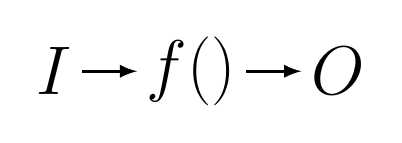
\begin{tikzpicture}
          [txt/.style={minimum width=2cm,anchor=center}
          ]
          \node (in) [fill=white, rounded corners] {\Huge $I$};

          \node (f) [fill=white
                    , rounded corners
                    , right=2em of in
                    ]
                    {\Huge $f()$};
          \node (out) [fill=white
                      , rounded corners
                      , right=2em of f
                      ]
                      {\Huge $O$};

          \draw[-latex,garr] (in) -- (f);
          \draw[-latex,garr] (f) -- (out);
      \end{tikzpicture}
    }%only
    \only<4->{
      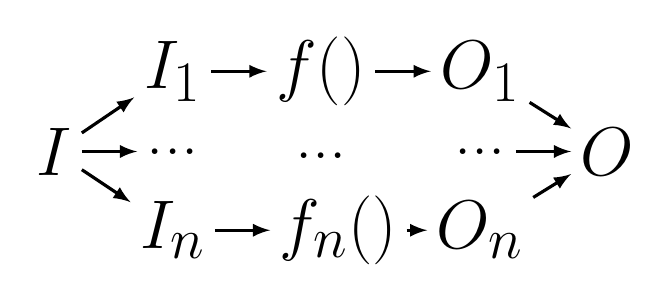
\begin{tikzpicture}
          [txt/.style={minimum width=2cm,anchor=center}
          ]
          \node (in1) [fill=white, rounded corners] {\Huge $I_1$};
          \node (inds) [fill=white
                      , below=1em of in1
                      , rounded corners] 
                            {\Huge ...};
          \node (bigi) [fill=white
                       , left=2em of inds
                       , rounded corners] 
                            {\Huge $I$};
          \node (inn) [fill=white
                      , below=1em of inds
                      , rounded corners] 
                            {\Huge $I_n$};


          \node (f1) [fill=white
                    , rounded corners
                    , right=2em of in1
                    ]
                    {\Huge $f()$};

          \node (fds) [fill=white
                    , rounded corners
                    , below=1em of f1
                    ]
                    {\Huge ...};
          \node (fn) [fill=white
                    , rounded corners
                    , right=2em of inn
                    ]
                    {\Huge $f_n()$};
          \node (out) [fill=white
                      , rounded corners
                      , right=2em of f1
                      ]
                      {\Huge $O_1$};

          \node (outds) [fill=white
                      , rounded corners
                      , below=1em of out
                      ]
                      {\Huge ...};
          \node (outn) [fill=white
                      , rounded corners
                      , below=1em of outds
                      ]
                      {\Huge $O_n$};
          \node (fout) [fill=white
                      , rounded corners
                      , right=2em of outds
                      ]
                      {\Huge $O$};

          \draw[-latex,garr] (in1) -- (f1);
          \draw[-latex,garr] (f1) -- (out);
          
          \draw[-latex,garr] (inn) -- (fn);
          \draw[-latex,garr] (fn) -- (outn);

          \draw[-latex,garr] (out) -- (fout);
          \draw[-latex,garr] (outds) -- (fout);
          \draw[-latex,garr] (outn) -- (fout);

          \draw[-latex,garr] (bigi) -- (in1);
          \draw[-latex,garr] (bigi) -- (inds);
          \draw[-latex,garr] (bigi) -- (inn);
      \end{tikzpicture}
    }
  \end{center}
  \note{
    \begin{itemize}
      \item Finally, I'll provide a discussion on the soundness of our approach
      \item Most of the thread-modular analysis builds upon the sequential
        abstract interpreter
      \item This is because each thread is, essentially, analyzed individually
        as a sequential program and then has its results propagated to other
        threads
      \item Our approach has its soundness based on this approach: we are just
        as sound as the underlying abstract interpreter 
      \item This is because we largely are not modifying the semantics of the
        sequential interpreter
      \item Specifically, our consideration of interference combinations in
        isolation is a form of focusing
      \item At a high level, focusing takes the input to the analysis and
        instead of analyzing the entire input it breaks it up into smaller
        pieces
      \item Each of these pieces are analyzed individually and then the results
        are combined
      \item Prior work has already discussed the soundness of this technique
        and we build of these findings
    \end{itemize}
  }
\end{frame}

\begin{frame}[fragile]{Handling Loops}
  \begin{columns}[c]
    \begin{column}{0.5\textwidth}
      \begin{lstlisting}[language=C, name=loop]
  int x = 0;
  void thread1() {
    create(thread2);
    while (...) {
      int t1 = x;
    }
    create(thread3);
  }
      \end{lstlisting}
    \end{column}
    \begin{column}{0.5\textwidth}
      \begin{lstlisting}[language=C, name=loop]
  void thread2() {
    x = 1;
    x = 2;
  }
  void thread3() {
    x = 10;
  }
      \end{lstlisting}
    \end{column}
  \end{columns}
  \pause
  \begin{itemize}[<+->]
    \item 0*1*2*
    \item $\Set{0,1,2}$
  \end{itemize}
  \note{
    \begin{itemize}
      \item Thus far, I've ignored the case where shared memory reads are
        performed within a loop
      \item In general, when a load is in a loop it can read from an arbitrary,
        and potentially infinite, number of different interferences
      \item As a result, if we simply treat loads within loops in the same way
        as as previously described there could be an infinite number of
        infinitely long combinations
      \item Consider this example, thread one creates thread two and then
        repeatedly loads the value of x an arbitrary number of times before
        creating thread two
      \item Notice that there is a must-happen-before edges between the load
        within the loop and the write to x by thread 3: because thread 3 is
        created after the load, the load cannot read the values written by
        thread 3
      \item So, the value read within the loop could be any sequence starting
        with an arbitrary number of zeros, followed by ones, followed by 2s
      \item Our previous system of constraints cannot handle such an infinite
        sequence so, instead, we merge all the potential interferences into a
        single value
      \item This means that the loads performed across loop-iterations will not
        be handled in a flow-sensitive way, but, any interfering store which
        cannot be read on any iteration will be remove thus improving acurracy
    \end{itemize}
  }
\end{frame}

\begin{frame}[fragile]{Property Directed Pruning}

  \begin{columns}[c]
    \begin{column}{0.5\textwidth}
    \begin{lstlisting}[language=C, name=motiv3]
int x = 0;
void thr(int v) {
  int t1 = 5 * v;
  int t2 = x;
  x = t1 + t2;
  if (t1 < 0) 
    ERROR!;
}
    \end{lstlisting}
    \end{column}
    \begin{column}{0.5\textwidth}
      \begin{lstlisting}[language=C, name=motiv3]
int main() {
  thread_create(thr,5);
  thread_create(thr,10);
  x = 1;
  thread_exit(0);
}

      \end{lstlisting}
    \end{column}
  \end{columns}
  \note{
    \begin{itemize}
      \item First, property directed pruning uses slices from the
        program-dependence graph to remove redundant statements
      \item If we look at this program, the main thread, on the right, creates
        two threads with arguments 5 and 10, and then performs a shared memory
        write to x
      \item The threads use their argument to perform a computation, and then
        perform a separate computation related to x
      \item The property being checked is related to t1, and the input argument
        to the thread
      \item If we look at the property being checking within each thread, it
        only depends on the input to the thread: the shared memory read on x
        has no influence on the reachability of the ERROR
      \item So, during the abstract interpretation, we can skip those
        statements involved with x
      \item Additionally, when exploring possible interference combinations, we
        can skip those related to x
      \item So, this both reduces the number of interference combinations and
        also reduces the individual analysis of each thread
      \item These dependencies between statements are captured easily by using
        the program dependence graph
    \end{itemize}
  }
\end{frame}

\begin{frame}[fragile]{Clustering}
  \begin{columns}[c]
    \begin{column}{0.5\textwidth}
    \begin{lstlisting}[language=C, name=prop]
int x = 0;
int y = 0;
void thread1() {
  x = 1;
  y = 1;
}
    \end{lstlisting}
    \end{column}
    \begin{column}{0.5\textwidth}
    \begin{lstlisting}[language=C, name=prop]
void thread2() {
  int t1 = x;
  int t2 = y;
  assert(x >= 0);
  assert(y >= 0);
}
    \end{lstlisting}
    \end{column}
  \end{columns}
  \pause
  \begin{itemize}[<+->]
    \item $2*2 = 4$ interference combinations
    \item Clustering: 2 combinations
  \end{itemize}
  \note{
    \begin{itemize}
      \item The second optimization we use is called clustering and also uses
        the program dependence graph
      \item This optimization reduces the number of possible interference
        combinations thereby reducing the runtime of the analysis
      \item Here we have two threads, one performing shared memory writes to
       x and y, and the other is performing shared memory read
      \item The two properties being analyzed are separately on x and y
      \item Using the previously described technique, there are two possible
        interfering stores for each of the loads in thread 2: one from thread 1
        and one causing thread 2 to read from its own memory environment
      \item This means that thread 2 will have to be analyzed 4 times, one for
        each combination
      \item However, if we look at the program, the properties being checked
        are performed on disjoint computations 
      \item Specifically, the writes to x and the writes to y do not influence
        each other
      \item So, during the analysis, the combinations between the reads of x
        and y in thread two can be performed independently
      \item As a result, we only need to consider the two combinations
        independently meaning we only need to run the analysis twice for thread
        two
    \end{itemize}
  }
\end{frame}


\end{document}
